\documentclass[12pt]{article}
\usepackage{amsmath, bm}
\usepackage{amssymb, amsthm, graphicx}
\usepackage{enumitem}
\usepackage{color}
\usepackage{float}
\usepackage[small]{caption}
\usepackage{subcaption}
\usepackage[mathscr]{euscript}
\usepackage{dsfont}
\usepackage{natbib}
\usepackage{amsmath}
\usepackage{placeins}
\usepackage{rotating}
\usepackage{pdflscape}
\makeatletter
\renewcommand{\eqref}[1]{\tagform@{\ref{#1}}}
\def\maketag@@@#1{\hbox{#1}}
\makeatother
\usepackage{bibentry}
\usepackage[hang,flushmargin]{footmisc} 
\usepackage{setspace}
\usepackage{titlesec}
%\usepackage{hyperref}
\titlespacing*{\section}{0pt}{5pt}{5pt}
\titlespacing*{\subsection}{0pt}{5pt}{5pt}
\parindent0pt

%\pdfminorversion=4
% NOTE: To produce blinded version, replace "0" with "1" below.
\newcommand{\blind}{0}

% DON'T change margins - should be 1 inch all around.
\addtolength{\oddsidemargin}{-.5in}%
\addtolength{\evensidemargin}{-1in}%
\addtolength{\textwidth}{1in}%
\addtolength{\textheight}{1.7in}%
\addtolength{\topmargin}{-1in}%


% General

\newcommand{\reals}{\mathbb{R}}
\newcommand{\integers}{\mathbb{Z}}
\newcommand{\naturals}{\mathbb{N}}

\newcommand{\pr}{\mathbb{P}}        % probability
\newcommand{\ex}{\mathbb{E}}        % expectation
\newcommand{\var}{\textnormal{Var}} % variance
\newcommand{\cov}{\textnormal{Cov}} % covariance

\newcommand{\law}{\mathcal{L}} % law of X
\newcommand{\normal}{N}        % normal distribution 

\newcommand{\argmax}{\textnormal{argmax}}
\newcommand{\argmin}{\textnormal{argmin}}

\newcommand{\ind}{\mathbbm{1}} % indicator function
\newcommand{\kernel}{K} % kernel function
\newcommand{\wght}{W} % kernel weight
\newcommand{\thres}{\pi} % threshold parameter


% Convergence

\newcommand{\convd}{\stackrel{d}{\longrightarrow}}              % convergence in distribution
\newcommand{\convp}{\stackrel{P}{\longrightarrow}}              % convergence in probability
\newcommand{\convas}{\stackrel{\textrm{a.s.}}{\longrightarrow}} % convergence almost surely
\newcommand{\convw}{\rightsquigarrow}                           % weak convergence


% Theorem-like declarations

\theoremstyle{plain}

\newtheorem{theorem}{Theorem}[section]
\newtheorem{prop}[theorem]{Proposition}
\newtheorem{lemma}[theorem]{Lemma}
\newtheorem{corollary}[theorem]{Corollary}
\newtheorem*{theo}{Theorem}
\newtheorem{propA}{Proposition}[section]
\newtheorem{lemmaA}[propA]{Lemma}
\newtheorem{definition}{Definition}[section]
\newtheorem{remark}{Remark}[section]
\renewcommand{\thelemmaA}{A.\arabic{lemmaA}}
\renewcommand{\thepropA}{A.\arabic{propA}}
\newtheorem*{algo}{Clustering Algorithm}


% Theorem numbering to the left

\makeatletter
\newcommand{\lefteqno}{\let\veqno\@@leqno}
\makeatother


% Heading

\newcommand{\heading}[2]
{  \setcounter{page}{1}
   \begin{center}

   \phantom{Distance to upper boundary}
   \vspace{0.5cm}

   {\LARGE \textbf{#1}}
   \vspace{0.4cm}
 
   {\LARGE \textbf{#2}}
   \end{center}
}


% Authors

\newcommand{\authors}[4]
{  \parindent0pt
   \begin{center}
      \begin{minipage}[c][2cm][c]{5cm}
      \begin{center} 
      {\large #1} 
      \vspace{0.05cm}
      
      #2 
      \end{center}
      \end{minipage}
      \begin{minipage}[c][2cm][c]{5cm}
      \begin{center} 
      {\large #3}
      \vspace{0.05cm}

      #4 
      \end{center}
      \end{minipage}
   \end{center}
}

%\newcommand{\authors}[2]
%{  \parindent0pt
%   \begin{center}
%   {\large #1} 
%   \vspace{0.1cm}
%      
%   #2 
%   \end{center}  
%}


% Version

\newcommand{\version}[1]
{  \begin{center}
   {\large #1}
   \end{center}
   \vspace{3pt}
} 








%\usepackage{xr}
%\externaldocument{supplement}



\begin{document}

\def\spacingset#1{\renewcommand{\baselinestretch}%
{#1}\small\normalsize} \spacingset{1}

\if0\blind
{
  \title{\bf Multiscale Comparison \\[0.1cm] of Nonparametric Trend Curves}
  \author{Marina Khismatullina\\ Erasmus School of Economics, Erasmus University Rotterdam\\
  and \\
  Michael Vogt\thanks{
  The authors gratefully acknowledge financial support by the Deutsche Forschungsgemeinschaft 
  (DFG, German Research Foundation), Germany – grant VO 2503/1-1, project number 430668955.}
  \hspace{.2cm}\\
  Department of Mathematics and Economics, Ulm University}
  \maketitle
} \fi

\if1\blind
{
  \bigskip
  \bigskip
  \bigskip
  \begin{center}
    {\LARGE\bf Multiscale Comparison \\[0.3cm] of Nonparametric Trend Curves}
\end{center}
  \medskip
} \fi

\bigskip
\begin{abstract}
{\noindent We develop new econometric methods for the comparison of nonparametric time trends. In many applications, practitioners are interested in examining the trending behaviour of the observed time series. Among other things, they would like to know which trends have a different form and in which time intervals the differences occur. We design a multiscale test to formally approach these questions. Specifically, we develop a test which allows to make rigorous confidence statements about which time trends are different and where (i.e., in which time intervals) they differ. Based on our multiscale test, we further develop a clustering algorithm which allows to cluster the observed time series into groups with the same trending behaviour. We derive asymptotic theory for our test and clustering methods. The theory is complemented by a simulation study and two applications to house pricing and GDP growth data.}
\end{abstract}

\noindent%
{\it Keywords:} Multiscale statistics; nonparametric regression; time series errors; strong approximations; anti-concentration bounds.
\vfill

\newpage
\spacingset{1.8} % DON'T change the spacing!

\numberwithin{equation}{section}
\allowdisplaybreaks[1]

\setlength{\abovedisplayskip}{3pt}
\setlength{\belowdisplayskip}{3pt}



\section{Introduction}\label{sec:intro}


The comparison of time trends is an important topic in time series analysis and has a wide range of applications in economics, finance and other fields such as climatology. In economics, one may for example wish to compare trends in real GDP \citep[][]{Grier1989} or trends in long-term interest rates \citep[][]{Christiansen1997} across different countries. In finance, it is of interest to compare the volatility trends of different stocks \citep[][]{Nyblom2000}. In climatology, researchers are interested in comparing temperature trends across different spatial locations \citep[][]{KarolyWu2005}. 


In this paper, we develop new econometric methods for the comparison of time trends. Classically, time trends are modelled stochastically in econometrics; see e.g.\ \cite{Stock1988}. Recently, however, there has been a growing interest in econometric models with deterministic time trends; see \cite{Cai2007}, \cite{Atak2011}, \cite{Robinson2012}, \cite{ChenGaoLi2012}, \cite{Zhang2012} and \cite{Hidalgo2014} among others. Following this recent development, we consider a general panel model with deterministic time trends. We observe a panel of $n$ time series $\mathcal{T}_i = \{(Y_{it}, \X_{it}): 1 \le t \le T \}$ of length $T$ for $1 \le i \le n$, where $Y_{it}$ are real-valued random variables and $\X_{it} = (X_{it,1},\ldots,X_{it,d})^\top$ are $d$-dimensional random vectors. Each time series $\mathcal{T}_i$ is modelled by the equation 
\begin{equation}\label{eq:model_full}
Y_{it} = m_i \Big( \frac{t}{T} \Big) + \bfbeta^\top_i \X_{it} + \alpha_i + \varepsilon_{it} 
\end{equation}
for $1 \le t \le T$, where $m_i: [0,1] \to \reals$ is a nonparametric (deterministic) trend function, $\bfbeta_i$ is a vector of $d$ parameters, $\X_{it}$ is a vector of covariates, $\alpha_i$ is a fixed effect and $\varepsilon_{it}$ is an idiosyncratic error term. As common in nonparametric regression, the trends $m_i$ in model \eqref{eq:model_full} depend on rescaled time $t/T$ rather than on real time $t$ and are thus defined on the unit interval $[0,1]$; see e.g.\ \cite{Robinson1989}, \cite{Dahlhaus1997} and \cite{VogtLinton2014} for a discussion of rescaled time. More details on the components of model \eqref{eq:model_full} together with the technical assumptions imposed on them can be found in Section \ref{sec:model}.


There are various statistical tests for the comparison of time trends in the literature. Most commonly, the null hypothesis $H_0: m_i = m + c_i \ \forall i \in \{1,\ldots,n\}$ is tested under which the trends $m_i$ are parallel to each other. By a simple normalization of the components in model \eqref{eq:model_full}, we can always achieve that the trends $m_i$ are exactly the same under $H_0$ rather than only parallel. Hence, after normalization (the details of which are given in Section \ref{sec:model}), the null hypothesis $H_0$ can be reformulated as follows: 
\[ H_0: m_1 = m_2 = \ldots = m_n. \]   
The problem of testing $H_0$ has been studied in a number of articles. In a restricted version of \eqref{eq:model_full} without covariates, it has been investigated in \cite{HaerdleMarron1990}, \cite{Hall1990}, \cite{DegrasWu2012} and \cite{ChenWu2018} among others. Test methods in a less restricted version of \eqref{eq:model_full} with covariates and homogeneous parameters ($\bfbeta_i = \bfbeta$ for all $i$) have been derived, e.g., in \cite{Zhang2012} and \cite{Hidalgo2014}.


Even though many different approaches for testing $H_0$ have been developed over the years, most of them have a serious shortcoming: they are very uninformative. They allow to say (with a certain statistical confidence) whether $H_0$ is violated or not, but they do not give any information on which types of violations occur. In particular, if $H_0$ is rejected, they only provide the information that some of the trend curves are not the same. Practitioners, however, would like to have much more specific information: they would like to know (i) \textit{which} trends have a different form and (ii) \textit{in which time intervals} the trends are different. The main aim of this paper is to construct a test procedure which provides exactly this information. More technically speaking, we construct a test which allows to make rigorous simultaneous confidence statements about (i) \textit{which} trend curves are different and (ii) \textit{where} (i.e., in which time intervals) they differ. 


Very roughly speaking, our approach works as follows: Let $\{\mathcal{I}_r: 1 \le r \le R\}$ be a large family of time intervals $\mathcal{I}_r \subseteq [0,1]$ and let $H_{0,r}^{[i,j]}: m_i(w) = m_j(w) \ \forall w \in \mathcal{I}_r$ be the hypothesis that the two trend curves $m_i$ and $m_j$ are identical on the interval $\mathcal{I}_r$. Our procedure simultaneously tests $H_{0,r}^{[i, j]}$ for all $r$ and all pairs of time series $(i,j)$. As the intervals $\mathcal{I}_r$ have different lengths or scales, it is called a multiscale method. Our main theoretical result shows that under suitable technical conditions, the developed multiscale test controls the familywise error rate, i.e., the probability of wrongly rejecting at least one null hypothesis $H_{0,r}^{[i, j]}$. As we will see, this allows us to make simultaneous confidence statements of the following form for a given significance level $\alpha \in (0,1)$: 
\textit{With probability at least $1-\alpha$, the trends $m_i$ and $m_j$ differ on any interval $\mathcal{I}_r$ and for any pair $(i,j)$ for which $H_{0,r}^{[i, j]}$ is rejected.} 
Hence, as desired, we can make confidence statements about (i) \textit{which} trend curves are different and (ii) \textit{where} they differ.


To the best of our knowledge, there are no other test procedures available in the literature which allow to make such confidence statements in the context of the general model \eqref{eq:model_full}. We are only aware of two other multiscale tests for the comparison of nonparametric time trends, both of which are restricted to a strongly simplified version of model \eqref{eq:model_full} without covariates. The first is a SiZer test by \cite{Park2009}, for which theory has only been derived in the special case of $n=2$ time series. The second is a multiscale test by \cite{KhismatullinaVogt2023}, which was developed to detect differences between epidemic time trends in the context of the COVID-19 pandemic. Being tailored to epidemic count data, their model is quite specific. In particular, it includes neither covariates nor fixed effects and it does not allow for any dependence structures across $i$ and $t$. In contrast, our model is quite general and thus apt for a wide range of economic and financial applications. Notably, our methodology can be regarded as an extension of that in \cite{KhismatullinaVogt2023}. However, their theoretical results heavily depend on the specific setting and thus do not carry over easily to our general framework. Our theoretical analysis is thus utterly different from theirs. See Remark \ref{remark:general-theo-2} for a discussion of the main differences. 


Our multiscale test is constructed step by step in Section \ref{sec:test} and its theoretical properties are laid out in Section \ref{sec:theo}. Based on this test, we further develop a clustering algorithm which allows to detect groups of time series with the same trend. This clustering algorithm is introduced and investigated in Section \ref{sec:clustering}. The proofs of all theoretical results are relegated to the Supplementary Material. We complement the theoretical analysis of the paper by a simulation study in Section A in the Supplement and two application examples in Section \ref{sec:app} and Section B of the Supplement. In the first application example, we examine a long record of housing price data from different countries, whereas the second example is concerned with GDP growth data from a number of OECD countries. 



\section{Model details}\label{sec:model}


\subsection{Notation}\label{subsec:model_notation}


For a vector $\mathbf{v} = (v_1, \ldots, v_m)\in\reals^m$, we write $\|\mathbf{v}\|_q = \big(\sum_{i=1}^m v_i^q\big)^{1/q}$ to denote its $\ell_q$-norm and use the shorthand $\|\mathbf{v}\| = \|\mathbf{v}\|_2$ in the special case $q = 2$. For a random variable $V$, we define its $\mathcal{L}^q$-norm by $\|V\|_q = (\ex |V|^q)^{1/q}$ and write $\|V\| := \|V\|_2$ in the case $q = 2$.
Let $\eta_t$ ($t \in \integers$) be independent and identically distributed ($\text{i.i.d.}$) random variables, write $\mathcal{F}_t  = (\ldots, \eta_{t-1}, \eta_t)$ and let $g: \reals^\infty \to \reals$ be a measurable function such that $g(\mathcal{F}_t) = g(\ldots, \eta_{t-1}, \eta_t)$ is a properly defined random variable. Following \cite{Wu2005}, we define the \textit{physical dependence measure} of the process $\{g(\mathcal{F}_t)\}_{t=-\infty}^\infty$ by $\delta_q(g, t) = \| g(\mathcal{F}_t) - g(\mathcal{F}_t^\prime) \|_q$, where $\mathcal{F}_t^\prime  = (\ldots, \eta_{-1}, \eta^\prime_0, \eta_1, \ldots, \eta_t)$ is a coupled version of $\mathcal{F}_t$ with $\eta_0^\prime$ an i.i.d.\ copy of $\eta_0$. 


\subsection{Model}\label{subsec:model_setting}


We now give some details on the components of model \eqref{eq:model_full}. We first have a closer look at the error structure which consists of the two components $\alpha_i$ and $\varepsilon_{it}$. We do not impose any distributional assumptions on the terms $\alpha_i$. In particular, they can be either deterministic or random and they may be correlated with the covariates $\X_{it}$ in an arbitrary way. Following the panel data literature in economics, we refer to them as fixed effects. The terms $\varepsilon_{it}$ are idiosyncratic errors which are assumed to have zero mean. They are allowed to be correlated across $t$ but are assumed to be independent across $i$. Precise technical conditions on them are given in Section \ref{subsec:model_assumptions} below.  Whereas the idiosyncratic errors $\varepsilon_{it}$ are restricted to be independent across $i$, we do not impose any restrictions on the dependence structure between the fixed effects $\alpha_i$ across $i$. Hence, we allow for cross-sectional dependence in the error structure via the fixed effects $\alpha_i$. Similarly, the covariates $\X_{it}$ are allowed to be dependent across $i$ in an arbitrary way. As a consequence, the $n$ time series $\mathcal{T}_i$ in our panel can be correlated with each other in various ways.  


The trend functions $m_i$ are not identified in model \eqref{eq:model_full}. In particular, equation \eqref{eq:model_full} is equivalent to $Y_{it} = m_i^\diamond(t/T) + \boldsymbol{\beta}_i^\top \boldsymbol{X}_{it} + \alpha_i^\diamond + \varepsilon_{it}$, where $m_i^\diamond = m_i + c_i^\diamond$, $\alpha_i^\diamond = \alpha_i - c_i^\diamond$ and $c_i^\diamond$ is an arbitrary real constant. 
For identification, we impose the constraint $\int_0^1 m_i(u) du = 0$ for all $i$, which vertically shifts each curve $m_i$ such that the overall mean level $\int_0^1 m_i(u)$ is equal to $0$. Such a normalization is quite natural in many application contexts. Take e.g.\ the application on house price data in Section \ref{sec:app}. The term $\int_0^1 m_i(u) du$ can be interpreted as the long-term average house price level in country $i$, which may be very different across countries. The normalization $\int_0^1 m_i(u) du = 0$ corrects for differences in these long-term price levels. Put differently, the normalized trends give the deviation from the long-term price levels. 


If the trends $m_i$ are parallel, i.e., $m_i = m + c_i$ with some constants $c_i$ and a common trend $m$ for all $i$, the constraint $\int_0^1 m_i(u) du = 0$ implies that $c_i = c := \int_0^1 m(u) du$ for all $i$. Put differently, it implies that the trends are exactly the same. Hence, under our identification constraint, the null hypothesis that the trends are parallel to each other coincides with the hypothesis that the trends are identical. 


Finally note that throughout the paper, we restrict attention to the case where the number of time series $n$ in model \eqref{eq:model_full} is fixed. Extending our theoretical results to the case where $n$ grows with $T$ is a possible topic for further research.


\subsection{Assumptions}\label{subsec:model_assumptions}


The error processes $\mathcal{E}_i = \{ \varepsilon_{it}: 1 \le t \le T\}$ satisfy the following conditions. 
\begin{enumerate}[label=(C\arabic*),leftmargin=1.05cm, itemsep=0pt, parsep=0pt, topsep=3pt]
\item \label{C-err1} 
The variables $\varepsilon_{it}$ allow for the representation $\varepsilon_{it} = g_i(\mathcal{F}_{it})$, where $\mathcal{F}_{it} = (\ldots,\eta_{it-2}, \linebreak \eta_{it-1},\eta_{it})$, the variables $\eta_{it}$ are i.i.d.\ across $t$, and $g_i: \reals^\infty \rightarrow \reals$ is a measurable function such that $\varepsilon_{it}$ is well-defined. It holds that $\ex[\varepsilon_{it}] = 0$ and $\| \varepsilon_{it} \|_q \le C < \infty$ for some $q > 4$ and a sufficiently large constant $C$. 
\item \label{C-err2} The processes $\mathcal{E}_i = \{ \varepsilon_{it}: 1 \le t \le T\}$ are independent across $i$.
\end{enumerate}
Assumption \ref{C-err1} implies that the error processes $\mathcal{E}_i$ are stationary and causal (in the sense that $\varepsilon_{it}$ does not depend on future innovations $\eta_{is}$ with $s>t$). The class of error processes that satisfy condition \ref{C-err1} is very large. It includes linear processes, nonlinear transformations thereof, as well as a large variety of nonlinear processes such as Markov chain models and nonlinear autoregressive models \citep[][]{Wu2016}. Following \cite{Wu2005}, we impose conditions on the dependence structure of the error processes $\mathcal{E}_i$ in terms of the physical dependence measure $\delta_q(g_i, t)$ defined in Section \ref{subsec:model_notation}: 
\begin{enumerate}[label=(C\arabic*),leftmargin=1.05cm, itemsep=0pt, parsep=0pt, topsep=3pt]
\setcounter{enumi}{2}
\item \label{C-err3} For each $i$, $\sum\nolimits_{s \ge 0} \delta_q(g_i, s)$ is finite and $\sum\nolimits_{s \ge t} \delta_q(g_i, s) = O ( t^{-\gamma} (\log t)^{-A})$ with $q$ from \ref{C-err1}, where $A > \frac{2}{3} (1/q + 1 + \gamma)$ and $\gamma = \{q^2 - 4 + (q-2) \sqrt{q^2 + 20q + 4}\} / 8q$. 
\end{enumerate}
For fixed $i$ and $t$, the expression $\sum\nolimits_{s \ge t} \delta_q(g_i, s)$ measures the cumulative effect of the innovation $\eta_0$ on the variables $\varepsilon_{it}, \varepsilon_{it+1},\ldots$ in terms of the $\mathcal{L}^q$-norm. Condition \ref{C-err3} puts some restrictions on the decay of $\sum\nolimits_{s \ge t} \delta_q(g_i, s)$ (as a function of $t$). It is fulfilled by a wide range of stationary processes $\mathcal{E}_i$. For a detailed discussion of \ref{C-err1}--\ref{C-err3} and some examples of error processes that satisfy these conditions, see \cite{KhismatullinaVogt2020}.


The covariates $\X_{it} = (X_{it,1},\ldots, X_{it, d})^\top$ are assumed to have the following properties. 
\begin{enumerate}[label=(C\arabic*),leftmargin=1.05cm, itemsep=0pt, parsep=0pt, topsep=3pt]
\setcounter{enumi}{3}
\item \label{C-reg1} It holds that $X_{it, j} = h_{ij}(\mathcal{G}_{it, j})$, where $\mathcal{G}_{it, j} = (\ldots, \xi_{it-1,j}, \xi_{it, j})$, the random variables $\xi_{it, j}$ are i.i.d.\ across $t$ and $h_{ij}: \reals^\infty \rightarrow \reals$ is a measurable function such that $X_{it, j}$ is well-defined. We use the notation $\X_{it} = \boldsymbol{h}_{i}(\mathcal{G}_{it})$ with $\boldsymbol{h}_i = (h_{i1}, \ldots, h_{id})^\top$ and $\mathcal{G}_{it} = (\mathcal{G}_{it,1}, \ldots, \mathcal{G}_{it, d})^\top$. It holds that $\ex [X_{it, j}]=0$ and $\| X_{it, j} \|_{q^\prime} <\infty$ for all $i$ and $j$, where $q^\prime > \max \{ 4, \theta q \}$ with $q$ from \ref{C-err1} and $\theta$ specified in \ref{C-grid} below.
\item \label{C-reg2} The matrix $\ex[\Delta \X_{it} \Delta \X_{it}^\top]$ is invertible for each $i$.
\item \label{C-reg3} For each $i$ and $j$, it holds that $\sum_{s \ge 0} \delta_{q^\prime}(h_{ij}, s)$ is finite and $\sum_{s \ge t} \delta_{q^\prime}(h_{ij}, s)= O(t^{-\alpha})$ for some $\alpha > 1/2 - 1/{q^\prime}$ with $q^\prime$ from \ref{C-reg1}.
\end{enumerate}
Assumption \ref{C-reg1} guarantees that the process $\{ \X_{it}: 1 \le t \le T \}$ is stationary and causal for each $i$. Assumption \ref{C-reg3} restricts the serial dependence of the process $\{ \X_{it}: 1 \le t \le T \}$ for each $i$ in terms of the physical dependence measure.


We finally impose some assumptions on the relationship between the covariates and the errors and on the trend functions $m_i$.
\begin{enumerate}[label=(C\arabic*),leftmargin=1.05cm, itemsep=0pt, parsep=0pt, topsep=3pt]
\setcounter{enumi}{6}
\item \label{C-reg-err} The random variables $\Delta \X_{it} = \X_{it} - \X_{it-1}$ and $\Delta \varepsilon_{it} = \varepsilon_{it} - \varepsilon_{it-1}$ are uncorrelated, i.e., $\cov(\Delta \X_{it}, \Delta \varepsilon_{it}) = \ex[\Delta \X_{it} \Delta \varepsilon_{it}] = 0$. 
\item \label{C-trend} The trend functions $m_i$ are Lipschitz continuous on $[0,1]$, i.e., $|m_i(v) - m_i(w)| \le L |v-w|$ for all $v,w \in [0,1]$ and some constant $L < \infty$. Moreover, they are normalised such that $\int_0^1m_i (u)du = 0$ for each $i$.
\end{enumerate}


%\begin{remark}
%Conditions \ref{C-reg1}--\ref{C-reg3} can be relaxed to cover locally stationary regressors. For example, \ref{C-reg1} may be replaced by
%\begin{enumerate}[label=(C\arabic*$^\prime$),leftmargin=1.1cm]
%\setcounter{enumi}{3}
%\item \label{C-reg1-star} The variables $X_{it, j}$ allow for the representation $X_{it, j} = h_{ij}(t; \mathcal{G}_{it, j})$, where $\mathcal{G}_{it, j} = (\ldots, \xi_{it-1,j}, \xi_{it, j})$, the random variables $\xi_{it, j}$ are i.i.d.\ across $t$ and $h_{ij}(t;\cdot): \reals^\infty \rightarrow \reals$ is a measurable function  for each $t$ such that $X_{it, j}$ is well-defined. We use the notation $\X_{it} = \boldsymbol{h}_{i}(t; \mathcal{G}_{it})$ with $\boldsymbol{h}_i = (h_{i1}, \ldots, h_{id})^\top$ and $\mathcal{G}_{it} = (\mathcal{G}_{it,1}, \ldots, \mathcal{G}_{it, d})^\top$. It holds that $\ex [X_{it, j}]=0$ and $\| X_{it, j} \|_{q^\prime} <\infty$ for all $i$, $j$ and $t$, where $q^\prime > \max \{ 4, \theta q \}$ with $q$ from \ref{C-err1} and $\theta$ specified in \ref{C-grid} below.
%\end{enumerate}
%The other assumptions can be adjusted accordingly. We conjecture that our main theoretical results still hold in this case. However, the complexity of the technical arguments will increase drastically. Hence, for the sake of clarity, we restrict attention to stationary covariates $\X_{it}$. 
%\end{remark}



\section{The multiscale test}\label{sec:test}


The strategy to construct our multiscale test is as follows: Let $\interval := [u-h, u+h] \subseteq [0,1]$ be the rescaled time interval with midpoint $u \in [0,1]$ and length $2h$. We call $u$ the location
and $h$ the scale of the interval $\interval$. For any given location-scale point $(u,h)$, let
\[ H_0^{[i, j]}(u, h): m_i(w) = m_j(w) \text{ for all } w \in \interval \] 
be the hypothesis that $m_i$ and $m_j$ are identical on the interval $\interval$. $H_0^{[i, j]}(u, h)$ can be viewed as a local null hypothesis that characterises the behaviour of two trend functions locally on the interval $\interval$, whereas $H_0: m_1 = m_2 = \ldots = m_n$ is the global null hypothesis that is concerned with the comparison of all trends on the whole time interval $[0, 1]$. We consider a large family of time intervals $\interval$ that fully cover the unit interval. More formally, we consider all intervals $\interval$ with $(u,h) \in \grid$, where $\grid$ is a set of location-scale points $(u,h)$ with the property that $\bigcup_{(u, h) \in \grid} \interval = [0,1]$. Technical conditions on the set $\grid$ as well as some examples are given below. The global null $H_0$ can now be formulated as 
\begin{align*}
H_0: \ & \text{The hypothesis } H_0^{[i, j]}(u, h) \text{ holds true for all intervals }  \interval \text{ with } (u, h) \in \grid \\[-0.075cm] & \text{and for all } 1 \le i < j \le n. 
\end{align*} 
This formulation shows that we can test $H_0$ by a procedure which simultaneously tests the local hypothesis $H_0^{[i, j]}(u, h)$ for all $1 \le i < j \le n$ and all $(u,h) \in \grid$. 


In what follows, we design such a simultaneous test procedure step by step. To start with, we introduce some auxiliary estimators in Section \ref{subsec:test:prep}. We then construct the test statistics in Section \ref{subsec:test:stat} and set up the test procedure in Section \ref{subsec:test:test}. Finally, Section \ref{subsec:test:impl} explains how to implement the procedure in practice. 


\subsection{Preliminary steps}\label{subsec:test:prep}


If the fixed effects $\alpha_i$ and the coefficient vectors $\bfbeta_i$ were known, our testing problem would be greatly simplified. In particular, we could consider the model
$Y_{it}^\circ = m_i (\frac{t}{T}) + \varepsilon_{it}$ with $Y_{it}^\circ := Y_{it} - \alpha_i - \bfbeta_i^\top \X_{it}$,
which is a standard nonparametric regression equation. As $\alpha_i$ and $\bfbeta_i$ are not observed in practice, we construct estimators $\widehat{\alpha}_i$ and $\widehat{\bfbeta}_i$ and replace the unknown variables $Y_{it}^\circ$ by the approximations $\widehat{Y}_{it} := Y_{it} -\widehat{\alpha}_i - \widehat{\bfbeta}_i^\top \X_{it}$. In what follows, we explain how to construct estimators of $\alpha_i$ and $\bfbeta_i$. 


In order to estimate the parameter vector $\bfbeta_i$ for a given $i$, we consider the time series $\Delta \mathcal{T}_i = \{(\Delta Y_{it}, \Delta \X_{it}): 2 \leq t \leq T\}$ of the first differences $\Delta Y_{it} = Y_{it} - Y_{i t-1}$ and $\Delta  \X_{it} =  \X_{it} - \X_{it-1}$. We can write $\Delta Y_{it} = Y_{it} - Y_{i t-1} =\bfbeta_i^\top \Delta \X_{it} + (m_i (\frac{t}{T}) - m_i (\frac{t-1}{T})) + \Delta \varepsilon_{it}$, where $ \Delta \varepsilon_{it} = \varepsilon_{it} - \varepsilon_{i t-1}$. Since $m_i$ is Lipschitz by Assumption \ref{C-trend}, we can use the fact that $ |m_i ( \frac{t}{T} ) - m_i (\frac{t-1}{T}) | = O(\frac{1}{T})$ to get that $\Delta Y_{it} = \bfbeta_i^\top \Delta \X_{it} + \Delta \varepsilon_{it} + O(\frac{1}{T})$. We may estimate $\bfbeta_i$ by applying least squares methods to this equation, treating $\Delta \X_{it}$ as the regressors and $\Delta Y_{it}$ as the response variable. As a result, we obtain the estimator
\begin{align}\label{eq:beta:est}
\widehat{\bfbeta}_i = \Big( \sum_{t=2}^T \Delta \X_{it} \Delta \X_{it}^\top \Big)^{-1} \sum_{t=2}^T \Delta \X_{it} \Delta Y_{it}.
\end{align}
In Lemma B.5 %\ref{lemma-beta-rate} 
in the Supplement, we show that $\widehat{\bfbeta}_i - \bfbeta_i = O_p(T^{-1/2})$ under our assumptions. Given $\widehat{\bfbeta}_i$, we next estimate the fixed effect term $\alpha_i$ by 
\begin{align}\label{eq:alpha:est}
\widehat{\alpha}_i &= \frac{1}{T}\sum_{t=1}^T \big(Y_{it} - \widehat{\bfbeta}_i^\top \X_{it}\big). 
\end{align}
This is a reasonable estimator of $\alpha_i$ for the following reason: For each $i$, it holds that $\widehat{\alpha}_i - \alpha_i = \big(\bfbeta_i - \widehat{\bfbeta}_i \big)^\top\frac{1}{T}\sum_{t=1}^T  \X_{it} + \frac{1}{T}\sum_{t=1}^T m_i(\frac{t}{T}) + \frac{1}{T}\sum_{t=1}^T \varepsilon_{it} = O_p(T^{-1/2})$, since $\frac{1}{T}\sum_{i=1}^T \varepsilon_{it} = O_p(T^{-1/2})$ by the law of large numbers, $\frac{1}{T}\sum_{i=1}^T m_i(t/T) = O(T^{-1})$ due to Lipschitz continuity of $m_i$ and the normalisation $\int_{0}^1 m_i(u)du = 0$, $\frac{1}{T}\sum_{t=1}^T  \X_{it} = O_p(1)$ by Chebyshev's inequality and $\widehat{\bfbeta}_i - \bfbeta_i = O_p (T^{-1/2})$. 


Besides $\widehat{\bfbeta}_i$ and $\widehat{\alpha}_i$, we also need an estimator of the long-run error variance $\sigma_i^2 = \sum\nolimits_{\ell=-\infty}^{\infty}$ $\cov(\varepsilon_{i0}, \varepsilon_{i\ell})$ for each $i$. Throughout the paper, we assume that the long-run error variance is the same for all $i$, i.e., $\sigma_i^2 = \sigma^2$ for all $i$.  For technical reasons, we nevertheless use a different estimator of $\sigma^2$ for each $i$. In particular, we let $\widehat{\sigma}_i^2$ be an estimator of $\sigma^2$ which depends only on the $i$-th time series $\{ \widehat{Y}_{it}: 1 \le t \le T \}$, i.e., $\widehat{\sigma}_i^2 = \widehat{\sigma}_i^2(\widehat{Y}_{i1},\ldots,\widehat{Y}_{iT})$ is a function of the variables $\widehat{Y}_{it}$ for $1 \le t \le T$.\footnote{This construction is for technical convenience. Specifically, it allows us to apply the strong approximation results from \cite{BerkesLiuWu2014} separately to each time series $i$, which simplifies the proofs.} Our theory works with any estimator $\widehat{\sigma}_i^2$ which has the property that $\widehat{\sigma}_i^2 = \sigma^2 + o_p(\rho_T)$ for each $i$, where $\rho_T$ slowly converges to zero, in particular, $\rho_T = o(1/\log T)$. We now briefly discuss two possible choices of $\widehat{\sigma}_i^2$. Following \cite{Kim2016}, we can estimate $\sigma^2$ by a variant of the subseries variance estimator, which was first proposed by \cite{Carlstein1986} and then extended by \cite{WuZhao2007}. A full definition of the estimator can be found in Lemma B.6 %\ref{lemmaA:lrv} 
of the Supplement where we derive its convergence rate. 
%Formally, we set
%\begin{align}
%\widehat{\sigma}_i^2 = \frac{1}{2(M-1)s_T}\sum_{m=1}^M \bigg[ \sum_{t = 1}^{s_T} & \Big(Y_{i(t + ms_T)} - Y_{i(t + (m-1)s_T)} \nonumber \\[-0.2cm] & - \widehat{\bfbeta}_i^\top\big(\X_{i(t+ms_T)} - \X_{i(t+(m-1)s_T)}\big) \Big)\bigg]^2, \label{eq:lrv}
%\end{align}
%where $s_T$ is the length of the subseries and $M = \lfloor T/s_T\rfloor$ is the largest integer not exceeding $T/s_T$. As per the optimality result in \cite{Carlstein1986}, we set $s_T \asymp T^{1/3}$. When implementing $\widehat{\sigma}_i^2$, we in particular choose $s_T = \lfloor T^{1/3}\rfloor$. According to  Lemma B.6 
%in the Supplement, $\widehat{\sigma}_i^2$ is an asymptotically consistent estimator of $\sigma_i^2$ with the rate of convergence $O_p(T^{-1/3})$. 
%The subseries estimator $\widehat{\sigma}_i^2$ 
The subseries estimator is completely nonparametric: it does not presuppose a specific time series model for the error process $\mathcal{E}_i = \{ \varepsilon_{it}: 1 \le t \le T\}$ but merely requires $\mathcal{E}_i$ to fulfill general weak dependence conditions. In practice, however, it often makes sense to impose additional structure on the error process $\mathcal{E}_i$. A very popular yet general error model is the class of $\text{AR}(\infty)$ processes. A difference-based estimator of the long-run error variance for this error model has been developed in \cite{KhismatullinaVogt2020} and can be easily adapted to the situation at hand. A detailed discussion of the estimator can be found in Section 4 of \cite{KhismatullinaVogt2020}. 


\subsection{Construction of the test statistics}\label{subsec:test:stat}


A statistic to test the local null hypothesis $H_0^{[i, j]}(u, h)$ for a given location-scale point $(u,h)$ and a given pair of time series $(i,j)$ can be constructed as follows: Let
\begin{align}
\widehat{\psi}_{ij, T}(u, h) = \sum\limits_{t=1}^T w_{t,T}(u, h)(\widehat{Y}_{it} - \widehat{Y}_{jt}) \label{eq:psi_hat_ij}
\end{align}
be a weighted average of the differenced variables $\widehat{Y}_{it} - \widehat{Y}_{jt}$. In particular, let $w_{t,T}(u, h)$ be kernel weights of the form
\begin{equation}\label{eq:weights}
w_{t,T}(u, h) = \frac{\Lambda_{t,T}(u, h)}{ \{\sum\nolimits_{t=1}^T \Lambda_{t,T}(u, h)^2 \}^{1/2} }, 
\end{equation}
where
\[ \Lambda_{t,T}(u, h) = K\Big(\frac{\frac{t}{T}-u}{h}\Big) \Big[ S_{T,2}(u, h) - \Big(\frac{\frac{t}{T}-u}{h}\Big) S_{T,1}(u, h) \Big], \]
$S_{T,\ell}(u, h) = (Th)^{-1} \sum\nolimits_{t=1}^T K(\frac{\frac{t}{T}-u}{h}) (\frac{\frac{t}{T}-u}{h})^\ell$ and $K$ is a kernel with the following properties: 
\begin{enumerate}[label=(C\arabic*),leftmargin=1.05cm,topsep=3pt]
\setcounter{enumi}{8}
\item \label{C-ker} The kernel $K$ is non-negative, symmetric about zero and integrates to one. Moreover, it has compact support $[-1,1]$ and is Lipschitz continuous, i.e., $|K(v) - K(w)| \le C_K |v-w|$ for any $v, w \in \reals$ and some constant $C_K > 0$.
\end{enumerate}
Note that the weights $w_{t,T}(u,h)$ are rescaled versions of the kernel weights of a standard local linear estimator \citep{FanGijbels1996}. Hence, the statistic $\widehat{\psi}_{ij, T}(u, h)$ is nothing else than a rescaled difference between local linear estimators of $m_i(u)$ and $m_j(u)$ with bandwidth $h$. It can thus be regarded as a measure of distance between the two trend curves $m_i$ and $m_j$ on the interval $\interval = [u-h, u+h]$. This suggests to use a normalized (absolute) version of $\widehat{\psi}_{ij, T}(u, h)$, in particular, the term 
\begin{equation}\label{eq:local-stat-without-correction}
\Big| \frac{\widehat{\psi}_{ij, T}(u, h)}{(\widehat{\sigma}_i^2 + \widehat{\sigma}_j^2)^{1/2}} \Big|
\end{equation}
as a statistic to test the local null $H_0^{[i, j]}(u, h)$. Our aim is to test $H_0^{[i, j]}(u, h)$ simultaneously for a wide range of location-scale points $(u,h)$ and all possible pairs of time series $(i,j)$. To take into account that we are faced with a simultaneous test problem, we replace the statistics from \eqref{eq:local-stat-without-correction} by additively corrected versions of the form 
\begin{align}\label{eq:psi_zero_ij}
\widehat{\psi}^0_{ij, T}(u, h) =  \Big|\frac{\widehat{\psi}_{ij, T}(u, h)}{(\widehat{\sigma}_i^2 + \widehat{\sigma}_j^2)^{1/2}}\Big| - \lambda(h),
\end{align}
where $\lambda(h) = \sqrt{2 \log \{ 1/(2h) \}}$. The scale-dependent correction term $\lambda(h)$ was first introduced in the multiscale approach of \cite{DuembgenSpokoiny2001} and has been used in various contexts since then. We refer to \citet{KhismatullinaVogt2020} for a detailed discussion of the idea behind this additive correction. 


In order to test the global null hypothesis $H_0$, we aggregate the test statistics $\widehat{\psi}^0_{ij, T}(u, h)$ by taking their maximum over all location-scale points $(u,h) \in \grid$ and all pairs of time series $(i,j)$ with $1 \le i < j \le n$. This leads to the multiscale test statistic 
\[ \widehat{\Psi}_{n,T} = \max_{(u,h) \in \grid, 1 \le i < j \le n} \widehat{\psi}^0_{ij, T}(u, h). \]
For our theoretical results, we suppose that the set of location-scale points $\grid$ is a subset of $\grid^{\text{full}} = \{ (u, h): \interval = [u-h,u+h] \subseteq [0,1]$ with $u = t/T$ and $h = s/T$  for some $1 \le t, s \le T$ and $h \in [h_{\min},h_{\max}] \}$ which fulfills the following conditions:
\begin{enumerate}[label=(C\arabic*),leftmargin=1.2cm, itemsep=0pt, parsep=0pt, topsep=3pt]
\setcounter{enumi}{9}

\item \label{C-grid} $|\mathcal{G}_T| = O(T^\theta)$ for some arbitrarily large but fixed constant $\theta > 0$, where $|\mathcal{G}_T|$ denotes the cardinality of $\mathcal{G}_T$. 

\item \label{C-h} $h_{\min} \gg T^{-(1-\frac{2}{q})} \log T$, i.e., $h_{\min} / \{ T^{-(1-\frac{2}{q})} \log T \} \rightarrow \infty$ with $q > 4$ defined in \ref{C-err1} and $h_{\max} = o(1)$.

\end{enumerate}
\ref{C-grid} and \ref{C-h} place relatively mild restrictions on the set $\grid$: \ref{C-grid} allows $\grid$ to be very large compared to the sample size $T$. In particular, $\grid$ may grow as any polynomial of $T$. \ref{C-h} allows $\grid$ to contain intervals $[u-h,u+h]$ of many different scales $h$, ranging from very small intervals of scale $h_{\min}$ to substantially larger intervals of scale $h_{\max}$.
As an example, we use the following grid in our application in Section \ref{sec:app}: $\mathcal{G}_T = U_T \times H_T$, where $U_T = \big\{ u \in [0,1]: u = \textstyle{\frac{t}{T}} \text{ with } 1 \le t \le T \big\}$ and $H_T = \big\{ h \in \big[ \textstyle{\frac{\log T}{T}}, \textstyle{\frac{1}{4}} \big]:  h = \textstyle{\frac{5t - 3}{T}} \text{ with } 1 \le t \le T \big\}$. We thus take into account all locations $u$ on an equidistant grid $U_T$ with step length $1/T$ and all scales $h=2/T, 7/T, 12/T,\ldots$ with $\log T /T \le h \le 1/4$. As we have yearly data, this implies that each interval $\interval =[u-h,u+h]$ with $(u,h) \in \grid$ spans $5, 15, 25, \ldots$ years. The lower bound $\log T / T$ is motivated by Assumption \ref{C-h}. 


\subsection{The test procedure}\label{subsec:test:test}


Let $\mathcal{M} = \{ (u,h,i,j): (u,h) \in \grid \text{ and } 1 \le i < j \le n \}$ be the collection of all location-scale points $(u,h)$ and all pairs of time series $(i,j)$ under consideration. Moreover, let $\mathcal{M}_0 \subseteq \mathcal{M}$ be the set of tuples $(u,h,i,j)$ for which $H_0^{[i, j]}(u, h)$ is true.
For a given significance level $\alpha \in (0,1)$, our multiscale test is carried out as follows: 
\begin{enumerate}[label=(\roman*),leftmargin=0.75cm,itemsep=0pt,parsep=0pt,topsep=3pt]

\item For each tuple $(u,h,i,j) \in \mathcal{M}$, we reject the local null hypothesis $H_0^{[i, j]}(u, h)$ if 
\[ \widehat{\psi}^0_{ij, T}(u, h) > q_{n,T}(\alpha), \]
where the critical value $q_{n,T}(\alpha)$ is constructed below such that the familywise error rate (FWER) is controlled at level $\alpha$. As usual, the FWER is defined as the probability of wrongly rejecting $H_0^{[i, j]}(u, h)$ for at least one tuple $(u,h,i,j) \in \mathcal{M}$. More formally, 
\[ \text{FWER}(\alpha) = \pr \Big( \exists (u,h,i,j) \in \mathcal{M}_0 : \widehat{\psi}^0_{ij, T}(u, h) > q_{n,T}(\alpha) \Big) \]
for a given significance level $\alpha \in (0,1)$ and we say that the FWER is controlled at level $\alpha$ if $\text{FWER}(\alpha) \le \alpha$.

\item We reject the global null hypothesis $H_0: m_1 = m_2 = \ldots = m_n$ if at least one local null hypothesis is rejected. Put differently, we reject $H_0$ if 
\[ \widehat{\Psi}_{n,T} > q_{n,T}(\alpha). \]

\end{enumerate}
We now construct a critical value $q_{n,T}(\alpha)$ which controls the FWER at level $\alpha$. Let $q_{n,T}(\alpha)$ be the $(1-\alpha)$-quantile of $\widehat{\Psi}_{n,T}$ under the global null $H_0: m_1 = m_2 = \ldots = m_n$. Since
\begin{align*} 
\text{FWER}(\alpha)
 & = 1 - \pr \Big( \forall (u,h,i,j) \in \mathcal{M}_0 : \widehat{\psi}^0_{ij, T}(u, h) \le q_{n,T}(\alpha) \Big) \\
 & = 1 - \pr \Big( \max_{ (u,h,i,j) \in \mathcal{M}_0} \widehat{\psi}^0_{ij, T}(u, h) \le q_{n,T}(\alpha) \Big) \\
 & \le 1 - \pr_{H_0} \Big( \max_{ (u,h,i,j) \in \mathcal{M}} \widehat{\psi}^0_{ij, T}(u, h) \le q_{n,T}(\alpha) \Big) \le \alpha 
\end{align*}
with $\pr_{H_0}$ denoting the probability under $H_0$, this choice of $q_{n,T}(\alpha)$ indeed controls the FWER at the desired level. However, this choice is not computable in practice. We thus replace it by a suitable approximation: Suppose we could perfectly estimate the parameter vector $\bfbeta_i$ and the long-run error variance $\sigma_i^2$ for each $i$ (where by assumption, $\sigma_i^2 = \sigma^2$ for all $i$), i.e., $\widehat{\bfbeta}_i = \bfbeta_i$ and $\widehat{\sigma}_i^2 = \sigma_i^2$ for each $i$. Then under $H_0$, the test statistics $\widehat{\psi}^0_{ij, T}(u, h)$ would simplify to 
\begin{equation}\label{eq:stat-idealized}
\widehat{\psi}^0_{ij, T}(u, h) = \Big| \frac{\sum\nolimits_{t=1}^T w_{t,T}(u, h) \{ (\varepsilon_{it} - \bar{\varepsilon}_i) - (\varepsilon_{jt} - \bar{\varepsilon}_j) \}}{(\sigma_i^2 + \sigma_j^2)^{1/2}} \Big| - \lambda(h), 
\end{equation}
where $\bar{\varepsilon}_i = \bar{\varepsilon}_{i,T} := T^{-1} \sum_{t=1}^T \varepsilon_{it}$ denotes the empirical average of the variables $\varepsilon_{i1},\ldots,\varepsilon_{iT}$. Replacing the error terms $\varepsilon_{it}$ in \eqref{eq:stat-idealized} by normally distributed variables leads to the statistics
\begin{align}\label{eq:phi_zero_ij}
\phi^0_{ij, T}(u, h) =  \bigg|\frac{\phi_{ij, T}(u, h)}{(\sigma_i^2 + \sigma_j^2)^{1/2}}\bigg| - \lambda(h)
\end{align}
with 
\begin{align}\label{eq:phi_ij}
\phi_{ij, T}(u, h) = \sum\limits_{t=1}^T w_{t,T}(u, h) \, \big\{ \sigma_i (Z_{it} - \bar{Z}_i) - \sigma_j (Z_{jt} - \bar{Z}_j) \big\},
\end{align}
where $Z_{it}$ are independent standard normal random variables for $1 \le t \le T$, $1 \le i \le n$ and we use the shorthand $\bar{Z}_i = \bar{Z}_{i,T} := T^{-1} \sum_{t=1}^T Z_{it}$. With this notation, we define 
\begin{align}\label{eq:Phi}
\Phi_{n,T} = \max_{1 \le i < j \le n}\max_{(u, h) \in \mathcal{G}_T} \phi^0_{ij, T}(u, h),
\end{align}
which can be regarded as a Gaussian version of the test statistic $\widehat{\Psi}_{n,T}$ under the null $H_0$ (in the idealized case with $\widehat{\bfbeta}_i = \bfbeta_i$ and $\widehat{\sigma}_i^2 = \sigma_i^2$ for all $i$). We now choose $q_{n,T}(\alpha)$ to be the $(1-\alpha)$-quantile of $\Phi_{n,T}$. 


%\begin{remark}
Importantly, this choice of $q_{n,T}(\alpha)$ can be computed by Monte Carlo simulations in practice: assuming that $\sigma_i^2 = \sigma^2$ for all $i$, we can rewrite the statistics from \eqref{eq:phi_zero_ij} as
\[\phi^0_{ij, T}(u, h) = \frac{1}{\sqrt{2}} \Big|\sum\limits_{t=1}^T w_{t,T}(u, h) \, \big\{ (Z_{it} - \bar{Z}_i) - (Z_{jt} - \bar{Z}_j) \big\}\Big| - \lambda(h). \] 
This shows that the distribution of these statistics and thus the distribution of the multiscale statistic $\Phi_{n,T}$ only depend on the Gaussian variables $Z_{it}$ for $1 \le i \le n$ and $1 \le t \le T$. Consequently, we can approximate the distribution of $\Phi_{n,T}$ -- and in particular its quantiles $q_{n,T}(\alpha)$ -- by simulating values of the Gaussian random variables $Z_{it}$. In Section \ref{subsec:test:impl}, we explain in detail how to compute Monte Carlo approximations of the quantiles $q_{n,T}(\alpha)$. 
%\end{remark}


\begin{remark}
Our test procedure can equivalently be formulated in terms of uniform confidence bands. To see this, let $\psi_{ij,T}(u,h) = \sum_{t=1}^T w_{t,T}(u,h) (m_i(\frac{t}{T}) - m_j(\frac{t}{T}))$ be a weighted local average of the difference between the functions $m_i$ and $m_j$ on the interval $\interval = [u-h,u+h]$ and define the random interval
$\textnormal{CI}_{ij,T}(u,h) = \Big[ \widehat{\psi}_{ij,T}(u,h) - c_{n,T}(\alpha,h), \widehat{\psi}_{ij,T}(u,h) + c_{n,T}(\alpha,h) \Big]$
for a given $\alpha \in (0,1)$, where $c_{n,T}(\alpha,h) = ( \widehat{\sigma}_i^2 + \widehat{\sigma}_j^2)^{1/2} (q_{n,T}(\alpha) + \lambda(h))$. $\textnormal{CI}_{ij,T}(u,h)$ can be regarded as a confidence interval for the parameter $\psi_{ij,T}(u,h)$ which is uniform over all $(u,h,i,j) \in \mathcal{M}$. In particular, our test rejects the local null hypothesis $H_0^{[i, j]}(u, h)$ at level $\alpha$ if and only if $0$ is not contained in the interval $\textnormal{CI}_{ij,T}(u,h)$. 
\end{remark}


\begin{remark} 
Our test is designed to control the FWER in contrast to other criteria such as the false discovery rate (FDR). The main reason for this is as follows: As formally shown in Section \ref{sec:theo},  FWER control allows us to make the following type of confidence statements:
\begin{equation}\label{eq:CS-FWER}
\begin{minipage}[c][2.25cm][c]{13cm}
With (asymptotic) probability $1-\alpha$, the differences between the trends detected by our test reflect true differences in the underlying trend curves.
\end{minipage}
\end{equation}
FDR control, in contrast, would only allow us to make the following type of statement:
\begin{equation}\label{eq:CS-FDR}
\begin{minipage}[c][2.25cm][c]{13cm}
On average, $100 (1-\alpha) \%$ of the differences detected by our test correspond to true differences.
\end{minipage}
\end{equation}
In our opinion, in most economic and financial applications, one is rather interested in statements of the form \eqref{eq:CS-FWER} than \eqref{eq:CS-FDR}. Take a financial example where the aim is to compare volatility trends of different stocks. Practitioners would like interpret the differences detected by the test. For instance, they would like to connect them to certain market events. This presupposes a certain confidence that the detected differences are worth interpreting (i.e., that they are not spurious but correspond to real differences). It is not enough to be confident that (on average) a certain percentage of the detected differences is worth interpreting. Hence, confidence statements of the form \eqref{eq:CS-FWER} appear more apt than statements of the form \eqref{eq:CS-FDR}.
\end{remark}
  

\subsection{Implementation of the test in practice}\label{subsec:test:impl}


In practice, we implement the test as follows for a given significance level $\alpha \in (0, 1)$:
\begin{enumerate}[label=\textit{Step \arabic*.}, leftmargin=1.45cm,itemsep=0pt,parsep=0pt,topsep=3pt]
\item Compute the $(1-\alpha)$-quantile $q_{n, T}(\alpha)$ of the Gaussian statistic $\Phi_{n,T}$ by Monte Carlo simulations. Specifically, draw a large number $L$ (say $L=5000$) of samples of independent standard normal random variables $\{Z_{it}^{(\ell)} : 1 \le t \le T, \, 1 \le i \le n \}$ for $1 \le \ell \le L$. For each sample $\ell$, compute the value $\Phi_{n,T}^{(\ell)}$ of the Gaussian statistic $\Phi_{n, T}$. Calculate the empirical $(1-\alpha)$-quantile $\widehat{q}_{n, T}(\alpha)$ from the values $\{ \Phi_{n, T}^{(\ell)}: 1 \le \ell \le L \}$ and use $\widehat{q}_{n, T}(\alpha)$ as an approximation of the quantile $q_{n, T}(\alpha)$.
\item For each $(i, j)$ with $1 \le i < j \le n$ and each $(u, h) \in \grid$, reject the local null hypothesis $H_0^{[i, j]}(u, h)$ if $\widehat{\psi}^0_{ij, T}(u, h)> \widehat{q}_{n, T}(\alpha)$. Reject the global null hypothesis $H_0$ if at least one local hypothesis $H_0^{[i, j]}(u, h)$ is rejected. 
\item Display the test results as follows. For each pair of time series $(i,j)$, let $\mathcal{S}^{[i, j]}(\alpha)$ be the set of intervals $\mathcal{I}_{u, h}$ for which we reject $H_0^{[i, j]}(u, h)$. Produce a separate plot for each pair ($i,j)$ which displays the intervals in $\mathcal{S}^{[i, j]}(\alpha)$. This gives a graphical overview over the intervals where our test finds a deviation from the null. 
\end{enumerate}


\pagebreak
\begin{remark} 
In some cases, the number of intervals in $\mathcal{S}^{[i, j]}(\alpha)$ may be quite large, rendering the visual representation of the test results outlined in Step 3 cumbersome. To overcome this drawback, we replace $\mathcal{S}^{[i, j]}(\alpha)$ with the subset of minimal intervals $\mathcal{S}^{[i, j]}_{\text{min}}(\alpha) \subseteq \mathcal{S}^{[i, j]}(\alpha)$. As in \cite{Duembgen2002}, we call an interval $\mathcal{I}_{u, h} \in \mathcal{S}^{[i, j]}(\alpha)$ minimal if there is no other interval $\mathcal{I}_{u^\prime, h^\prime} \in \mathcal{S}^{[i, j]}(\alpha)$ such that $\mathcal{I}_{u^\prime, h^\prime} \subset \mathcal{I}_{u, h}$. Notably, our theoretical results remain to hold true when the sets $\mathcal{S}^{[i, j]}(\alpha)$ are replaced by $\mathcal{S}^{[i, j]}_{\text{min}}(\alpha)$. See Section \ref{sec:theo} for the details. 
\end{remark}



\section{Theoretical properties of the multiscale test}\label{sec:theo}


To start with, we investigate the auxiliary statistic
\begin{align}\label{eq:Phi_hat}
\widehat{\Phi}_{n,T} = \max_{1 \le i < j \le n}  \max_{(u, h) \in \mathcal{G}_T} \widehat{\phi}^0_{ij, T}(u, h),
\end{align}
where
\begin{equation*}
\widehat{\phi}^0_{ij, T}(u, h) =\bigg| \frac{\widehat{\phi}_{ij, T}(u, h)} {\{ \widehat{\sigma}_i^2 + \widehat{\sigma}_j^2 \}^{1/2}} \bigg| - \lambda(h)
\end{equation*}
and
\begin{align*}
\widehat{\phi}_{ij, T}(u, h) 
 & = \sum_{t=1}^T w_{t,T}(u, h) \big\{ (\varepsilon_{it} - \bar{\varepsilon}_i) + (\bfbeta_i - \widehat{\bfbeta}_i)^\top (\X_{it} - \bar{\X}_{i}) \\[-0.4cm]
 & \phantom{= \sum_{t=1}^T w_{t,T}(u, h) \big\{} - (\varepsilon_{jt} - \bar{\varepsilon}_j) -  (\bfbeta_j - \widehat{\bfbeta}_j)^\top (\X_{jt} - \bar{\X}_{j}) \big\}
\end{align*}
with $\bar{\varepsilon}_i = \bar{\varepsilon}_{i,T} := T^{-1} \sum_{t=1}^T \varepsilon_{it}$ and $\bar{\X}_{i} =  \bar{\X}_{i, T} := T^{-1}\sum_{t=1}^T  \X_{it}$. By construction, it holds that $\widehat{\phi}_{ij, T}(u, h) = \widehat{\psi}_{ij, T}(u, h)$ under $H_0^{[i, j]}(u, h)$. Hence, the auxiliary statistic $\widehat{\Phi}_{n,T}$ is identical to the multiscale test statistic $\widehat{\Psi}_{n,T}$ under the global null $H_0$.
%To determine the distribution of the test statistic $\widehat{\Psi}_{n,T}$ under $H_0$, it thus suffices to study the auxiliary statistic $\widehat{\Phi}_{n,T}$.
The following theorem is key for deriving theoretical properties of our multiscale test. It shows that the distribution of the auxiliary statistic $\widehat{\Phi}_{n,T}$ is close to the distribution of the Gaussian statistic $\Phi_{n,T}$ introduced in \eqref{eq:Phi}. 
\begin{theorem}\label{theo:stat:global}
Let \ref{C-err1}--\ref{C-h} be fulfilled. Moreover, assume that $\widehat{\sigma}_i^2 = \sigma_i^2 + o_p(\rho_T)$ with $\rho_T = o(1/\log T)$ and $\sigma_i^2 = \sigma^2$ for all $i$. Then  
\begin{equation*}
\sup_{x \in \reals} \big| \pr(\widehat{\Phi}_{n, T} \le x) - \pr(\Phi_{n,T} \le x) \big| = o(1).
\end{equation*}
\end{theorem}


\begin{remark}\label{remark:general-theo-1}
The proof of Theorem \ref{theo:stat:global} builds on two important theoretical results: strong approximation theory for dependent processes \citep{BerkesLiuWu2014} and anti-concentration bounds for Gaussian random vectors \citep{Nazarov2003}. It can be regarded as a further development of the proof strategy in \cite{KhismatullinaVogt2020} who developed multiscale methods to test for local increases/decreases of the nonparametric trend function $m$ in the univariate time series model $Y_t = m(t/T) + \varepsilon_t$. We extend their theoretical results in several directions: we consider the case of multiple time series, we allow for a  flexible fixed effect error structure and we include covariates, which produces additional approximation error that is quite technical to handle (see Step 4 in the proof of Theorem \ref{theo:stat:global} for the details). 
\end{remark}


\begin{remark}\label{remark:general-theo-2}
Even though the multiscale test in \cite{KhismatullinaVogt2023} is similar in spirit to ours, their theoretical analysis is completely different from ours. In particular, their proofs build on high-dimensional central limit theorems for hyperrectangles \citep{Chernozhukov2017}, while our proofs rely on strong approximations. Hence, even without the inclusion of covariates and fixed effects, our proof strategy would be completely different. The issue is that the arguments in \cite{KhismatullinaVogt2023} rely heavily on the i.i.d.\ structure of the data and thus do not carry over to the model setting at hand which involves complicated dependence structures both across $i$ and $t$.
\end{remark}


With the help of Theorem \ref{theo:stat:global}, we now examine the theoretical properties of our multiscale test developed in Section \ref{sec:test}. The following proposition shows that our test of the global null $H_0$ has correct (asymptotic) size.
\begin{prop}\label{prop:test}
Let the conditions of Theorem \ref{theo:stat:global} be satisfied. Then under $H_0$, 
\[ \pr \big( \widehat{\Psi}_{n,T} \le q_{n,T}(\alpha) \big) = (1 - \alpha) + o(1). \]
\end{prop}
The next proposition characterises the power of the test against a certain class of local alternatives. To formulate it, we consider a sequence of pairs of functions $m_ i := m_{i,T}$ and $m_ j := m_{j,T}$ that depend on the time series length $T$ and that are locally sufficiently far from each other.
\begin{prop}\label{prop:test:power}
Let the conditions  of Theorem \ref{theo:stat:global} be satisfied. Moreover, assume that for some pair of indices $i$ and $j$, the functions $m_ i = m_{i,T}$ and $m_ j = m_{j,T}$ have the following property: There exists $(u, h) \in \mathcal{G}_T$ with $[u-h, u+h] \subseteq [0,1]$ such that $m_{i,T}(w) - m_{j,T}(w) \ge c_T \sqrt{\log T/(Th)}$ for all $w \in [u-h, u+h]$ or $m_{j,T}(w) - m_{i,T}(w) \ge c_T \sqrt{\log T/(Th)}$ for all $w \in [u-h, u+h]$, where $\{c_T\}$ is any sequence of positive numbers with $c_T \rightarrow \infty$. Then 
\[ \pr \big( \widehat{\Psi}_{n,T} \le q_{n,T}(\alpha) \big) = o(1). \]
\end{prop}


We now turn attention to the local null hypotheses $H_0^{[i, j]}(u, h)$. As already defined above, let $\mathcal{M} = \{ (u,h,i,j): (u,h) \in \grid \text{ and } 1 \le i < j \le n \}$ be the collection of location-scale points $(u,h)$ and pairs of time series $(i,j)$ under consideration. Moreover, let $\mathcal{M}_0 \subseteq \mathcal{M}$ be the set of tuples $(u,h,i,j)$ for which $H_0^{[i, j]}(u, h)$ is true. Since we test $H_0^{[i, j]}(u, h)$ simultaneously for all $(u,h,i,j) \in \mathcal{M}$, we would like to bound the probability of making at least one false discovery. More formally, we would like to control the family-wise error rate 
\begin{align*} 
\text{FWER}(\alpha) 
 & = \pr \Big(\exists \,  (u,h,i,j) \in \mathcal{M}_0: \widehat{\psi}^0_{ij, T}(u, h) > q_{n,T}(\alpha) \Big) \\
 & = \pr \Big(\exists \,  (u,h,i,j) \in \mathcal{M}_0: \interval \in \mathcal{S}^{[i, j]}(\alpha) \Big)
\end{align*}
at level $\alpha$, where $\mathcal{S}^{[i, j]}(\alpha)$ is the set of intervals $\interval$ for which $H_0^{[i, j]}(u, h)$ is rejected. The following result shows that our test asymptotically controls the FWER at level $\alpha$.
\begin{prop}\label{prop:test:fwer}
Under the conditions of Theorem \ref{theo:stat:global}, for any given $\alpha \in (0,1)$, 
\[ \textnormal{FWER}(\alpha) \leq \alpha + o(1). \]
\end{prop}
The statement of Proposition \ref{prop:test:fwer} can obviously be reformulated as follows: 
\begin{align*}
\pr\Big( \forall \, (u,h,i,j) \in \mathcal{M} \text{ for which } H_0^{[i, j]}(u, h) \text{ is true, } H_0^{[i, j]}(u, h) & \text{ is not rejected} \Big) \\ & \quad \ge 1 - \alpha + o(1).
\end{align*}
Consequently, we can make the following simultaneous confidence statement: 
\begin{equation}\label{eq:CS-v1}
\begin{minipage}[c][2.25cm][c]{13cm}
\textit{With (asymptotic) probability at least $1-\alpha$, the trends $m_i$ and $m_j$ differ on any interval $\interval$ and for all pairs $(i,j)$ for which $H_0^{[i, j]}(u, h)$ is rejected.}
\end{minipage}
\end{equation}
Put differently:
\begin{equation}\label{eq:CS-v2}
\begin{minipage}[c][2.25cm][c]{13cm}
\textit{With (asymptotic) probability at least $1-\alpha$, for any pair $(i,j)$ with $1 \le i < j \le n$, the two trends $m_i$ and $m_j$ differ on all intervals $\interval \in \mathcal{S}^{[i, j]}(\alpha)$.}
\end{minipage}
\end{equation}


\begin{remark}
According to \eqref{eq:CS-v2}, the graphical device introduced in Section \ref{subsec:test:impl} which depicts the intervals in $\mathcal{S}^{[i, j]}(\alpha)$ comes with the following statistical guarantee: we can claim with (asymptotic) confidence at least $1-\alpha$ that the trends $m_i$ and $m_j$ differ on all the depicted intervals. As $\mathcal{S}^{[i, j]}_{\textnormal{min}}(\alpha) \subseteq \mathcal{S}^{[i, j]}(\alpha)$ for all $i$ and $j$, this guarantee remains to hold true when the sets $\mathcal{S}^{[i, j]}(\alpha)$ are replaced by the sets of minimal intervals $\mathcal{S}_{\textnormal{min}}^{[i, j]}(\alpha)$.
\end{remark}



\section{Clustering}\label{sec:clustering}


Consider a situation in which the null $H_0: m_1 = m_2 = \ldots = m_n$ is violated. Even though some of the trend functions are different in this case, part of them may still be the same. Put differently, there may be groups of time series which have the same time trend. Formally speaking, we define a group structure as follows: There exist sets or groups of time series $G_1,\ldots, G_N$ with $N \le n$ and $\{1,\ldots, n\} = \mathbin{\dot{\bigcup}}_{\ell=1}^{N} G_\ell$ such that for each $1 \le \ell \le N$,
$m_i = f_\ell$ for all $i \in G_\ell$, 
where $f_\ell$ are group-specific trend functions. Hence, the time series which belong to the group $G_\ell$ all have the same time trend $f_\ell$. Throughout the section, we suppose that the group-specific trend functions $f_\ell$ have the following properties: 
\begin{enumerate}[label=(C\arabic*),leftmargin=1.2cm,topsep=3pt]
\setcounter{enumi}{11}
\item \label{C-clustering} For each $\ell$, $f_\ell = f_{\ell,T}$ is a Lipschitz continuous function with $\int_0^1 f_{\ell,T}(w) dw = 0$. In particular, $|f_{\ell,T}(v) - f_{\ell,T}(w)| \le L |v-w|$ for all $v, w \in [0,1]$ and some constant $L < \infty$ that does not depend on $T$. Moreover, for any $\ell \ne \ell^\prime$, the trends $f_{\ell,T}$ and $f_{\ell^\prime,T}$ differ in the following sense: There exists $(u, h) \in \mathcal{G}_T$ with $\interval \subseteq [0,1]$ such that $f_{\ell,T}(w) - f_{\ell^\prime,T}(w) \ge c_T \sqrt{\log T/(Th)}$ for all $w \in \interval$ or $f_{\ell^\prime,T}(w) - f_{\ell,T}(w) \ge c_T \sqrt{\log T/(Th)}$ for all $w \in \interval$, where $0 < c_T \rightarrow \infty$.
\end{enumerate}


In what follows, we combine our multiscale methods with a clustering algorithm to estimating the unknown group structure from the data. More specifically, we use the multiscale statistics $\max_{(u, h) \in \mathcal{G}_T}\hat{\psi}^0_{ij, T}(u, h)$ calculated for each $i$ and $j$ as distance measures which are fed into a hierarchical clustering algorithm. To describe the algorithm, let $S \subseteq \{1,\ldots, n\}$ and $S^\prime \subseteq \{1,\ldots, n\}$ be two sets of time series from our sample. We define a dissimilarity measure between $S$ and $S^\prime$ by 
\begin{equation}\label{dissimilarity}
\widehat{\Delta}(S,S^\prime) = \max_{\substack{i \in S, \\ j \in S^\prime}} \Big(\max_{(u, h) \in \mathcal{G}_T}\hat{\psi}^0_{ij, T}(u, h)\Big) 
\end{equation}
%This is called a complete linkage measure of dissimilarity. Alternatively, we may work with an average or a single linkage measure. We now combine the dissimilarity measure $\widehat{\Delta}$
and run the following hierarchical agglomerative clustering (HAC) algorithm: 
\vspace{3pt}

\noindent \textit{Step $0$ (Initialisation):} Let $\widehat{G}_i^{[0]} = \{ i \}$ denote the $i$-th singleton cluster for $1 \le i \le n$ and define $\{\widehat{G}_1^{[0]},\ldots,\widehat{G}_n^{[0]} \}$ to be the initial partition of time series into clusters. 

\noindent \textit{Step $r$ (Iteration):} Let $\widehat{G}_1^{[r-1]},\ldots,\widehat{G}_{n-(r-1)}^{[r-1]}$ be the $n-(r-1)$ clusters from the previous step. Determine the pair of clusters $\widehat{G}_{\ell}^{[r-1]}$ and $\widehat{G}_{{\ell}^\prime}^{[r-1]}$ for which 
\[ \widehat{\Delta}(\widehat{G}_{\ell}^{[r-1]},\widehat{G}_{{\ell}^\prime}^{[r-1]}) = \min_{1 \le k < k^\prime \le n-(r-1)} \widehat{\Delta}(\widehat{G}_{k}^{[r-1]},\widehat{G}_{k^\prime}^{[r-1]}) \]  
and merge them into a new cluster. 
\vspace{3pt}

\noindent Iterating this procedure for $r = 1,\ldots, n-1$ yields a tree of nested partitions $\{\widehat{G}_1^{[r]},\ldots,\widehat{G}_{n-r}^{[r]}\}$, which can be graphically represented by a dendrogram. Roughly speaking, the HAC algorithm merges the $n$ singleton clusters $\widehat{G}_i^{[0]} = \{ i \}$ step by step until we end up with the cluster $\{1,\ldots, n\}$. In each step, the closest two clusters are merged, where the distance between clusters is measured in terms of the dissimilarity $\widehat{\Delta}$. We refer the reader to Section 14.3.12 in \cite{HastieTibshiraniFriedman2009} for an overview of hierarchical clustering methods. 


When the number of groups $N$ is known, we estimate the group structure $\{G_1,\ldots, G_N\}$ by the $N$-partition $\{\widehat{G}_1^{[n-N]},\ldots,\widehat{G}_{N}^{[n-N]}\}$ produced by the HAC algorithm. When $N$ is unknown, we estimate it by the $\widehat{N}$-partition $\{\widehat{G}_1^{[n-\widehat{N}]},\ldots,\widehat{G}_{\widehat{N}}^{[n-\widehat{N}]}\}$, where 
\[ \widehat{N} = \min \Big\{ r = 1,2,\ldots \Big| \max_{1 \le \ell \le r} \widehat{\Delta} \big( \widehat{G}_\ell^{[n-r]} \big) \le q_{n,T}(\alpha) \Big\} \]
is an estimator of $N$. In the definition of $\widehat{N}$, we write $\widehat{\Delta}(S) = \widehat{\Delta}(S,S)$ for short and let $q_{n,T}(\alpha)$ be the $(1-\alpha)$-quantile of $\Phi_{n,T}$ defined in Section \ref{subsec:test:test}. 


The following proposition summarises the theoretical properties of the estimators $\widehat{N}$ and $\{ \widehat{G}_1,\ldots,\widehat{G}_{\widehat{N}} \}$, where we use the shorthand $\widehat{G}_\ell = \widehat{G}_\ell^{[n-\widehat{N}]}$ for $1 \le \ell \le \widehat{N}$. 
\begin{prop}\label{prop:clustering:1}
Let the conditions of Theorem \ref{theo:stat:global} and \ref{C-clustering} be satisfied. Then 
\[ \pr \Big( \big\{ \widehat{G}_1,\ldots,\widehat{G}_{\widehat{N}} \big\} = \{ G_1,\ldots, G_N \} \Big) \ge (1-\alpha) + o(1) \]
and $\pr ( \widehat{N} = N ) \ge (1-\alpha) + o(1)$. 
\end{prop}
This result allows us to make confidence statements about the estimated clusters $\{ \widehat{G}_1,\ldots, $ $\widehat{G}_{\widehat{N}} \}$ and their number $\widehat{N}$. In particular, we can claim with asymptotic confidence at least $1 - \alpha$ that the estimated group structure is identical to the true group structure. 
%Note that it is possible to let the significance level $\alpha$ depend on the sample size $T$ in Proposition \ref{prop:clustering:1}. In particular, we can allow $\alpha = \alpha_T$ to converge slowly to zero as $T \rightarrow \infty$, in which case we obtain that $\pr ( \{ \widehat{G}_1,\ldots,\widehat{G}_{\widehat{N}} \} = \{ G_1,\ldots, G_N \} ) \rightarrow 1$ and $\pr ( \widehat{N} = N ) \rightarrow 1$. 
%The proof of Proposition \ref{prop:clustering:1} can be found in the Supplement.


Our multiscale methods do not only allow us to compute estimators of the unknown groups $G_1,\ldots, G_N$ and their number $N$. They also provide information on the locations where two group-specific trend functions $f_\ell$ and $f_{\ell^\prime}$ differ from each other. To turn this claim into a mathematically precise statement, we need to introduce some notation. First of all, note that the indexing of the estimators $\widehat{G}_1,\ldots,\widehat{G}_{\widehat{N}}$ is completely arbitrary. We could, for example, change the indexing according to the rule $\ell \mapsto \widehat{N} - \ell + 1$. In what follows, we suppose that the estimated groups are indexed such that $P( \widehat{G}_\ell = G_\ell \text{ for all } \ell ) \ge (1-\alpha) + o(1)$. Proposition \ref{prop:clustering:1} implies that this is possible without loss of generality. Keeping this convention in mind, we define the sets 
\begin{align*}
\mathcal{A}_{n,T}^{[\ell,\ell^\prime]}(\alpha) & = \Big\{ (u, h) \in \mathcal{G}_T: \widehat{\psi}^0_{ij, T}(u, h) > q_{n,T}(\alpha) \text{ for some } i \in \widehat{G}_\ell, j \in \widehat{G}_{\ell^\prime} \Big\} \\
\mathcal{S}^{[\ell,\ell^\prime]}_{n, T}(\alpha) & = \big\{ \interval = [u-h, u+h]: (u, h) \in \mathcal{A}_{n,T}^{[\ell,\ell^\prime]}(\alpha) \big\}
\end{align*}
for $1 \le \ell < \ell^\prime \le \widehat{N}$. An interval $\interval$ is contained in $\mathcal{S}^{[\ell,\ell^\prime]}_{n, T}(\alpha)$ if our multiscale test indicates a significant difference between the trends $m_i$ and $m_j$ on the interval $\interval$ for some $i \in \widehat{G}_\ell$ and $j \in \widehat{G}_{\ell^\prime}$. Put differently, $\interval \in \mathcal{S}^{[\ell,\ell^\prime]}_{n, T}(\alpha)$ if the test suggests a significant difference between the trends of the $\ell$-th and the $\ell^\prime$-th group on the interval $\interval$. We further let
\[ E_{n,T}^{[\ell,\ell^\prime]}(\alpha) = \Big\{ \forall \interval \in \mathcal{S}^{[\ell,\ell^\prime]}_{n, T}(\alpha): f_\ell(v) \ne f_{\ell^\prime}(v) \text{ for some } v \in \interval = [u-h, u+h] \Big\} \]
be the event that the group-specific time trends $f_\ell$ and $f_{\ell^\prime}$ differ on all intervals $\interval \in \mathcal{S}^{[\ell,\ell^\prime]}_{n, T}(\alpha)$. With this notation at hand, we can make the following formal statement.  
\begin{prop}\label{prop:clustering:2}
Under the conditions of Proposition \ref{prop:clustering:1}, the event 
\[ E_{n,T}(\alpha) = \Big\{ \bigcap_{1 \le \ell < \ell^\prime \le \widehat{N}} E_{n,T}^{[\ell,\ell^\prime]}(\alpha) \Big\} \cap \Big\{ \widehat{N} = N \text{ and } \widehat{G}_\ell = G_\ell \text{ for all } \ell \Big\} \]
asymptotically occurs with probability at least $1-\alpha$, i.e., 
$\pr ( E_{n,T}(\alpha) ) \ge (1 - \alpha) + o(1)$. 
\end{prop}
According to Proposition \ref{prop:clustering:2}, the sets $\mathcal{S}^{[\ell,\ell^\prime]}_{n, T}(\alpha)$ allow us to locate, with a pre-specified confidence, time intervals where the group-specific trend functions $f_\ell$ and $f_{\ell^\prime}$ differ from each other. In particular, we can claim with asymptotic confidence at least $1 - \alpha$ that the trend functions $f_\ell$ and $f_{\ell^\prime}$ differ on all intervals $\interval \in \mathcal{S}^{[\ell,\ell^\prime]}_{n, T}(\alpha)$.\footnote{This statement remains to hold true when the sets of intervals $\mathcal{S}^{[\ell,\ell^\prime]}_{n, T}(\alpha)$ are replaced by the corresponding sets of minimal intervals.} 

\section{Empirical application}\label{sec:app}


We analyse a historical dataset on nominal annual house prices from \cite{Knoll2017} that contains data for $14$ advanced economies covering $143$ years from $1870$ to $2012$. 
A second application on GDP growth is provided in the Supplement. 
In our analysis, we consider 8 countries (Australia, Belgium, Denmark, France, Netherlands, Norway, Sweden and USA) over the time period 1890--2012. The data for all these countries except Belgium contain no missing values. The data for Belgium have five missing values (spanning five years during WWI) 
%\footnote{The missing values in the Belgium time series span five years during World War I.} 
which we impute by linear interpolation. The time series of the other $6$ countries have more than $10$ missings each, which is why we exclude them from the analysis.


We deflate the nominal house prices with the corresponding consumer price index (CPI) to obtain real house prices ($HP$). Variables that can potentially influence the average house prices are numerous, and there seems to be no general consensus about what the main determinants are. Possible determinants include, but are not limited to, demographic factors such as population growth (\citealt{Holly2010}, \citealt{Wang2014}, \citealt{Churchill2021}); fundamental economic factors such as real GDP (\citealt{Huang2013}, \citealt{Churchill2021}), interest rate and inflation (\citealt{Abelson2005}, \citealt{Otto2007}, \citealt{Huang2013}, \citealt{Jorda2015}); urbanisation (\citealt{Chen2011}, \citealt{Wang2017}); government subsidies and regulations (\citealt{Malpezzi1999}); stock markets (\citealt{Gallin2006}); etc. In our analysis, we focus on the following determinants of the average house prices: real GDP ($GDP$), population size ($POP$), long-term interest rate ($I$) and inflation ($INFL$) which is measured as change in CPI. Most other factors (such as government regulations, construction costs, and real wages) vary rather slowly over time and can be captured by time trend, fixed effects and slope heterogeneity.
Data for CPI, real GDP, population size and long-term interest rate are taken from the Jordà-Schularick-Taylor Macrohistory Database\footnote{See \cite{Jorda2017} for a detailed description of the variable construction.}, which is freely available at \url{http://www.macrohistory.net/data/} (accessed on 13 January 2022).


In summary, we observe a panel of $n = 8$ time series $\mathcal{T}_i = \{(Y_{it}, \X_{it}): 1 \le t \le T \}$ of length $T = 123$ for each country $i \in \{1,\ldots, 8\}$, where $Y_{it} = \ln HP_{it}$ and $\X_{it} = (\ln GDP_{it}, \ln POP_{it}, I_{it}, INFL_{it})^\top$. For each $i$, the time series $\mathcal{T}_i$ is assumed to follow the model $Y_{it} = m_i(t/T) + \bfbeta^\top_i \X_{it} + \alpha_i + \varepsilon_{it}$, or equivalently, 
\begin{equation}\label{eq:model:app4}
\ln HP_{it} =  m_i \Big( \frac{t}{T} \Big) + \beta_{i, 1} \ln GDP_{it} + \beta_{i, 2} \ln POP_{it} + \beta_{i, 3} I_{it} + \beta_{i, 4} INFL_{it} + \alpha_i + \varepsilon_{it}
\end{equation}
for $1 \le t \le T$, where $\bfbeta_i = (\beta_{i, 1}, \beta_{i, 2}, \beta_{i, 3}, \beta_{i, 4})^\top$ is a vector of unknown parameters, $m_i$ is a country-specific unknown nonparametric time trend and $\alpha_i$ is a fixed effect. 


The inclusion of a nonparametric trend function $m_i$ in model \eqref{eq:model:app4} is supported by the literature. \cite{Ugarte2009}, for example, model the trend in average Spanish house prices by means of splines. \cite{Winter2022} include a long-term stochastic trend component when describing the dynamic behaviour of real house prices in $8$ advanced economies. Including a nonparametric trend function when modelling the evolution of house prices is also the main conclusion in \cite{Zhang2016}, where it is shown that the time series of logarithmic US house prices is trend-stationary, i.e., can be transformed into a stationary series by subtracting a deterministic trend.


We implement our multiscale test as follows: 
(i) We choose $K$ to be the Epanechnikov kernel and consider the set of location-scale points $\mathcal{G}_T = U_T \times H_T$, where $U_T = \{ u \in [0,1]: u = \textstyle{\frac{t}{T}} \text{ with } 1 \le t \le T \}$ and $H_T = \{ h \in [ \textstyle{\frac{\log T}{T}}, \textstyle{\frac{1}{4}} ]:  h = \textstyle{\frac{5t - 3}{T}} \text{ with } 1 \le t \le T \}$. We thus take into account
%all locations $u$ on an equidistant grid $U_T$ with step length $1/T$ and
all scales $h=2/T, 7/T, 12/T,\ldots$ with $\log T /T \le h \le 1/4$, where the lower bound $\log T / T$ is motivated by Assumption \ref{C-h}. This implies that each interval $\interval =[u-h,u+h]$ with $(u,h) \in \grid$ spans $5, 15, 25, \ldots$ years.   
(ii) We assume that for each $i$, the error process $\mathcal{E}_i = \{\varepsilon_{it}: 1 \leq t \leq T\}$ follows an AR($p_i$) model and we estimate the long-run variances $\sigma_i^2$ by the difference-based estimator from \cite{KhismatullinaVogt2020} with tuning parameters $q$ and $r$ equal to $15$ and $10$, respectively. We choose $p_i$ by minimizing BIC. For $7$ out of $8$ countries the order $p_i$ determined by BIC\footnote{Applying other information criteria such as FPE, AIC and HQ yields exactly the same results in these cases.} is equal to $1$. For the sake of simplicity, we thus assume that $p_i = 1$ for all $i$.
(iii) The critical values $q_{n, T}(\alpha)$ are computed by Monte Carlo methods as described in Section \ref{subsec:test:impl}, where we set $L=5000$.
Besides these choices, we implement the test exactly as described in Section \ref{sec:test}.  


\begin{sidewaysfigure}[p!]
\begin{minipage}[t]{0.24\textwidth}
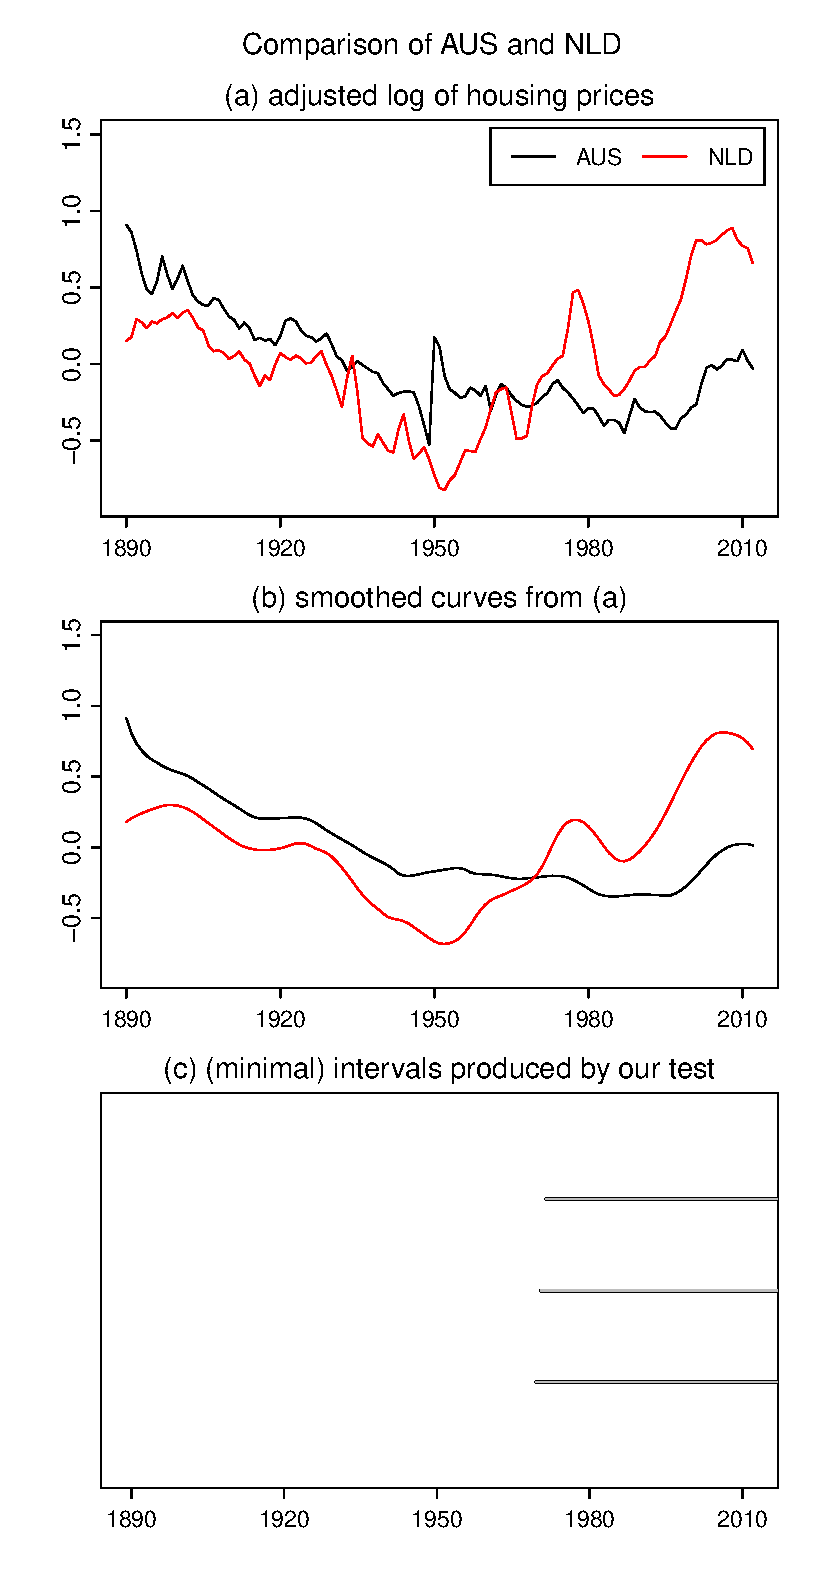
\includegraphics[width=\textwidth]{output/plots/hp/AUS_vs_NLD}
\caption{Test results for the comparison of the house prices in Australia and the Netherlands.}\label{fig:hp:Australia:Netherlands}
\end{minipage}
\hspace{0.1cm}
\begin{minipage}[t]{0.24\textwidth}
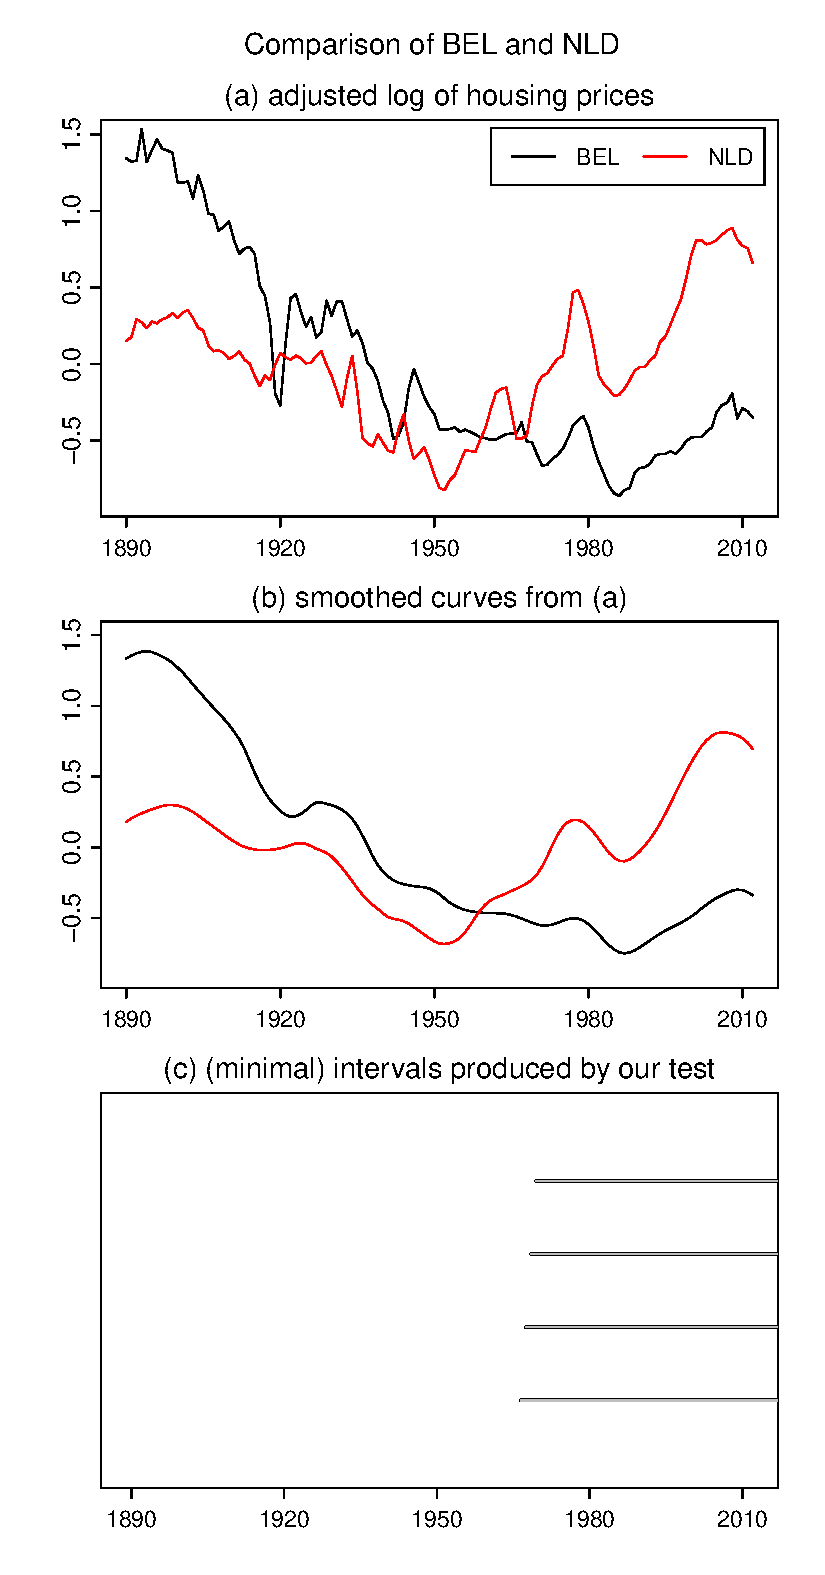
\includegraphics[width=\textwidth]{output/plots/hp/BEL_vs_NLD}
\caption{Test results for the comparison of the house prices in Belgium and the Netherlands.}\label{fig:hp:Belgium:Netherlands}
\end{minipage}
\hspace{0.1cm}
\begin{minipage}[t]{0.24\textwidth}
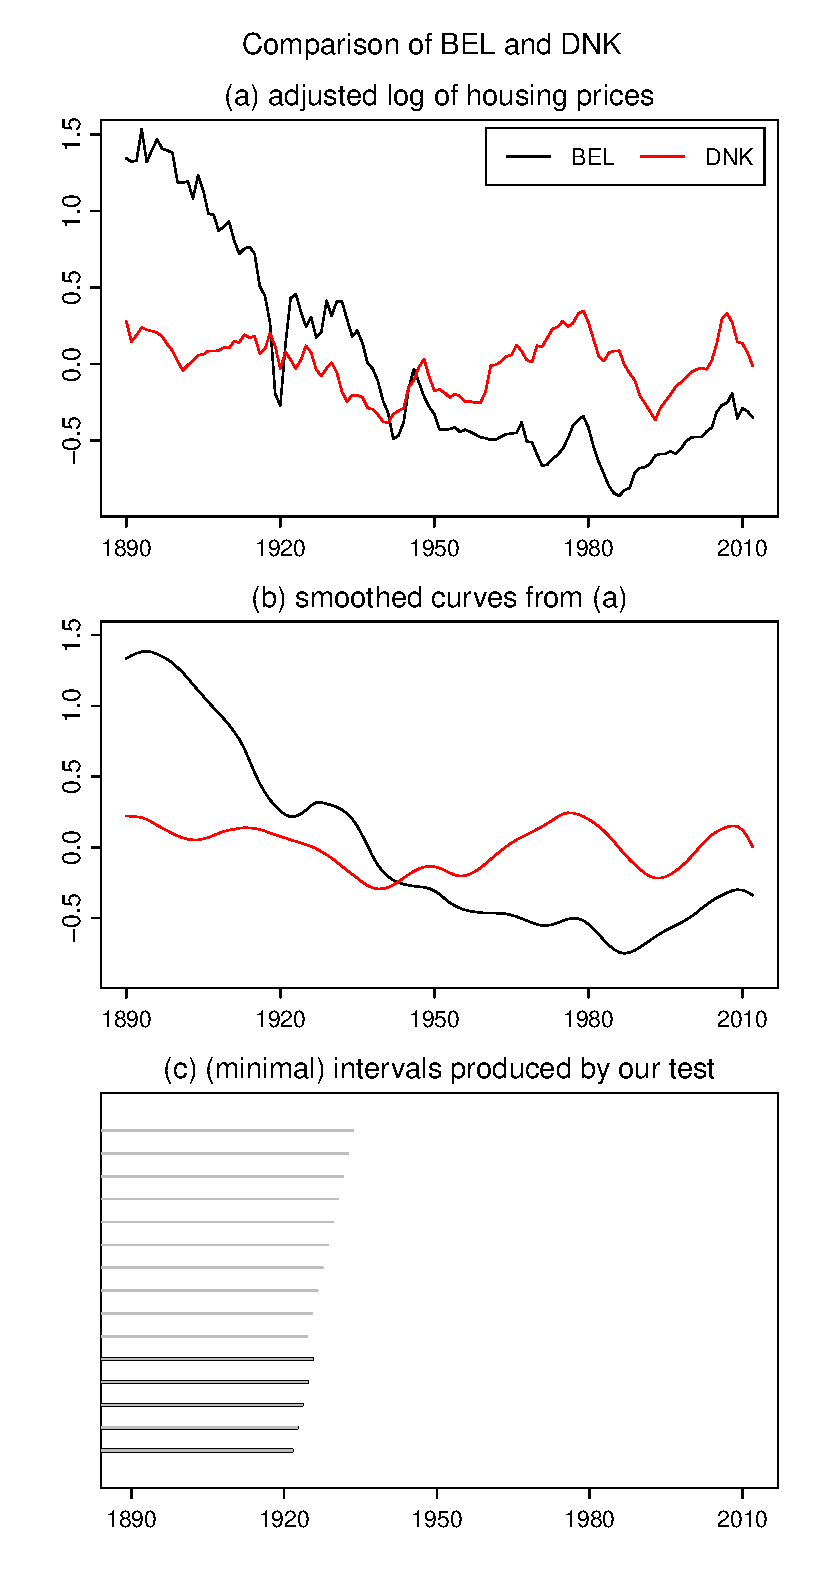
\includegraphics[width=\textwidth]{output/plots/hp/BEL_vs_DNK}
\caption{Test results for the comparison of the house prices in Belgium and Denmark.}\label{fig:hp:Belgium:Denmark}
\end{minipage}
\hspace{0.1cm}
\begin{minipage}[t]{0.24\textwidth}
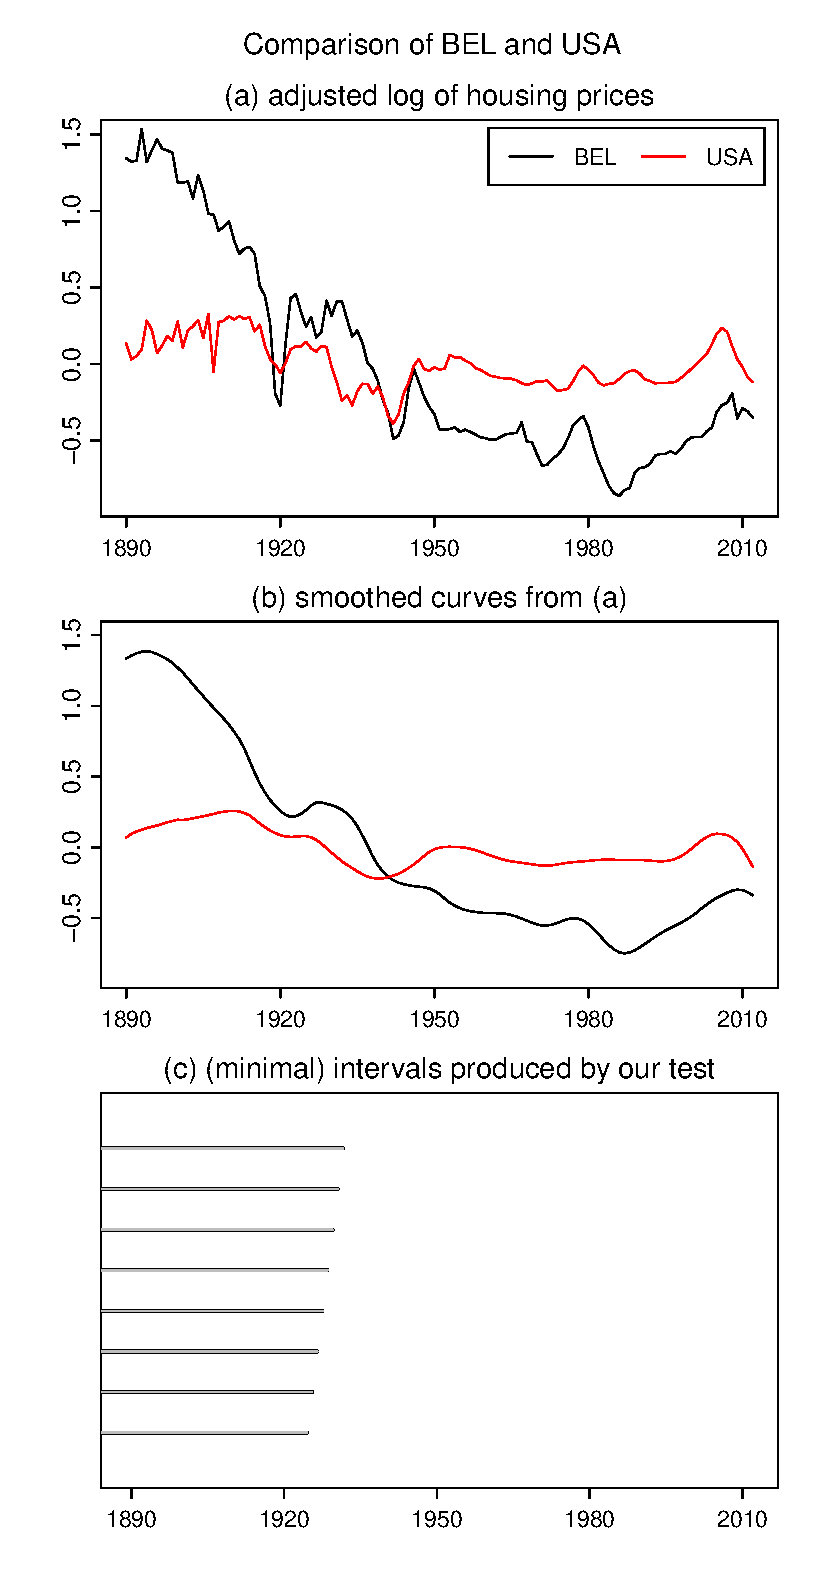
\includegraphics[width=\textwidth]{output/plots/hp/BEL_vs_USA}
\caption{Test results for the comparison of the house prices in Belgium and the USA.}\label{fig:hp:Belgium:USA}
\end{minipage}
\caption*{Note: In each figure, panel (a) shows the two augmented time series of the house prices, panel (b) presents smoothed versions of the augmented time series, and panel (c) depicts the set of intervals $\mathcal{S}^{[i, j]}(\alpha)$ in grey and the subset of minimal intervals $\mathcal{S}^{[i, j]}_{min}(\alpha)$ in black.}
\end{sidewaysfigure}


We are now ready to apply the test to the data. The overall null $H_0$ is rejected at levels $\alpha = 0.05$ and $\alpha = 0.1$. The detailed test results for $\alpha =0.05$ are presented in Figures \ref{fig:hp:Australia:Netherlands}--\ref{fig:hp:Belgium:USA}. 
Each figure corresponds to a specific pair of countries $(i, j)$ for which our test detects differences between the trends. 
%As in Section \ref{subsec:app:gdp}, each figure corresponds to the comparison of a pair of countries $(i, j)$ for which our test detects differences between the trends. 
In each figure, panel (a) shows the augmented time series $\{\widehat{Y}_{it}: 1 \le t \le T\}$ and $\{\widehat{Y}_{jt}: 1 \le t \le T\}$ for the two countries $i$ and $j$ that are compared. 
Panel (b) presents smoothed versions of the time series from (a), in particular, it shows local linear kernel estimates of the two trend functions $m_i$ and $m_j$, where the bandwidth window covers $15$ years and an Epanechnikov kernel is used.
Panel (c) presents the results produced by our test: 
it depicts in grey the set $\mathcal{S}^{[i, j]}(\alpha)$ of all the intervals for which the test rejects the local null $H_0^{[i, j]}(u, h)$. The set of minimal intervals $\mathcal{S}^{[i, j]}_{min}(\alpha) \subseteq \mathcal{S}^{[i, j]}(\alpha)$ is highlighted in black. According to \eqref{eq:CS-v2}, we can make the following simultaneous confidence statement about the intervals plotted in panels (c) of Figures \ref{fig:hp:Australia:Netherlands}--\ref{fig:hp:Belgium:USA}: we can claim, with confidence of about $95\%$, that there is a difference between the functions $m_i$ and $m_j$ on each of these intervals. 


%Panel (a) shows the augmented time series $\{\widehat{Y}_{it}: 1 \le t \le T\}$ and $\{\widehat{Y}_{jt}: 1 \le t \le T\}$ for the two countries $i$ and $j$ under consideration. Panel (b) presents smoothed versions of the time series from (a) with the bandwidth window covering $15$ years. Panel (c) presents the test results for the level $\alpha=0.05$. As before, the set of intervals $\mathcal{S}^{[i, j]}(\alpha)$ for which our test rejects and the set of minimal intervals $\mathcal{S}^{[i, j]}_{min}(\alpha) \subseteq \mathcal{S}^{[i, j]}(\alpha)$ are depicted in grey and black, respectively. According to \eqref{eq:CS-v2}, we can make the following simultaneous confidence statement about the intervals plotted in panels (c) of Figures \ref{fig:hp:Australia:Netherlands}--\ref{fig:hp:Belgium:USA}: we can claim, with confidence of about $95\%$, that there is a difference between the trends $m_i$ and $m_j$ on each of these intervals. 


Overall, our findings are in line with the observations in \cite{Knoll2017} who find considerable cross-country heterogeneity in the house price trends. The authors note that before World War II, the countries exhibit similar trends in real house prices, while the trends start to diverge sometime after World War II. This fits with our findings in Figures \ref{fig:hp:Australia:Netherlands}--\ref{fig:hp:Belgium:Netherlands} which show that our test detects differences between the trends of Australia and the Netherlands (of Belgium and the Netherlands) starting only from 1968 (1966) onwards. Contrary to \cite{Knoll2017}, however, our test also finds significant differences in the first half of the observed time period, specifically, between the time trends of Belgium and Denmark and of Belgium and the USA (Figures \ref{fig:hp:Belgium:Denmark} and \ref{fig:hp:Belgium:USA}, respectively). This discrepancy in the results is most certainly due to the fact that the method used in \cite{Knoll2017} does not account for effects of other factors such as GDP or population growth, while our test allows to include various determinants of the average house prices in model \eqref{eq:model:app4}. We in particular believe that the rate of population growth is the main factor that causes the discrepancy in the results. The influence of this factor on house prices greatly varies across countries. Specifically, the estimated regression coefficient of the population growth rate for Belgium (BEL), Denmark (DNK) and the USA is $\widehat{\beta}_{\text{BEL}, 2} = 3.45$, $\widehat{\beta}_{\text{DNK}, 2} = 0.19$ and $\widehat{\beta}_{\text{USA}, 2} = 0.80$, respectively. To substantiate our conjecture, we have repeated the analysis from Section 7 with one distinction: we do not include the population growth rate as a regressor in the model. As expected, our test does not find any significant differences between Belgium and Denmark and between Belgium and the USA in this case, which is in line with the findings presented in \cite{Knoll2017}. 


\begin{figure}[t!]
\begin{center}
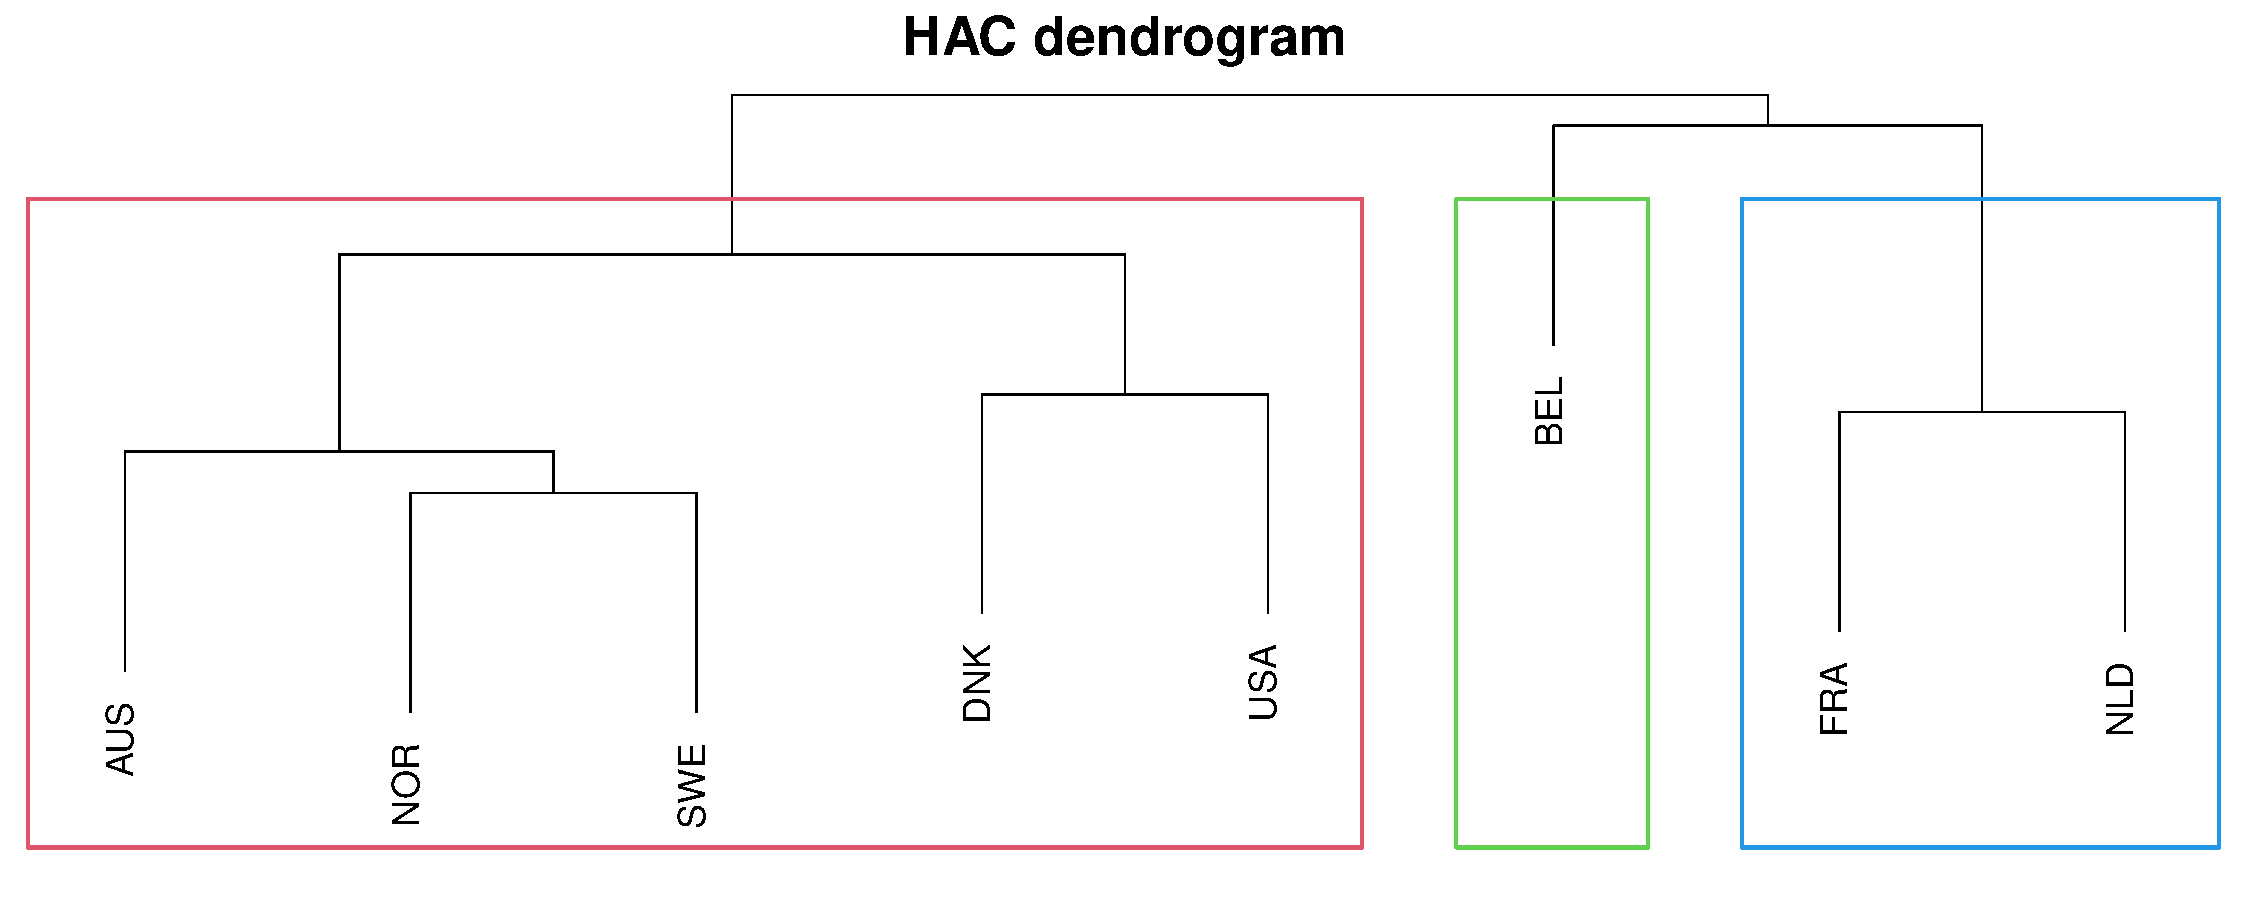
\includegraphics[width=0.75\textwidth]{output/plots/hp/dendrogram}
\caption{Dendrogram of the HAC algorithm. Each coloured rectangle corresponds to one of the clusters.}\label{fig:hp:dend}

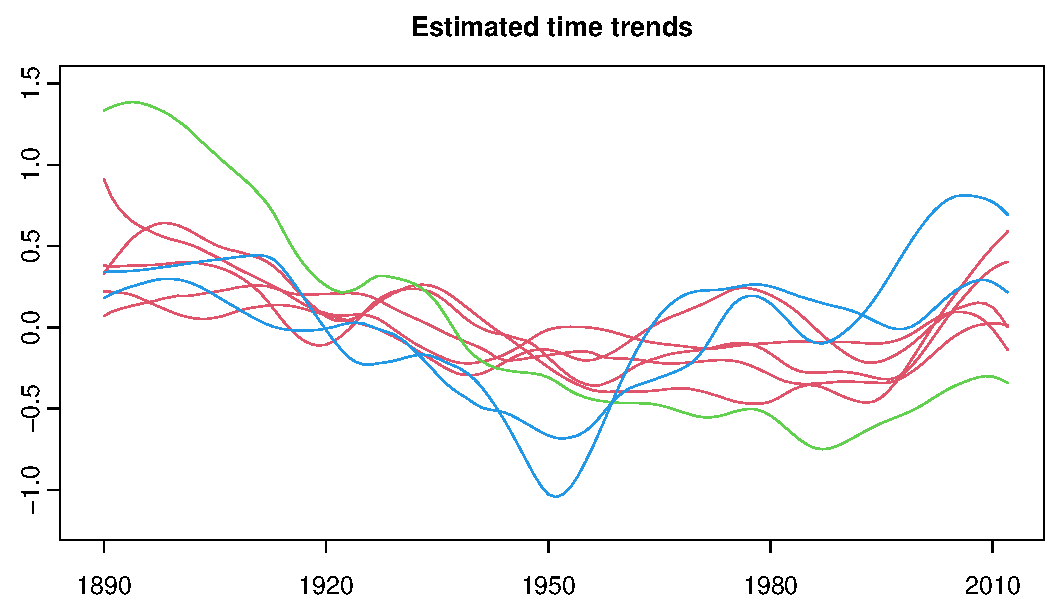
\includegraphics[width=0.75\textwidth]{output/plots/hp/all_clusters}
\caption{Local linear estimates of the $n=8$ time trends (calculated from the augmented time series $\widehat{Y}_{it}$ with a bandwidth window covering $15$ years and an Epanechikov kernel). Each trend estimate is coloured according to the cluster that it is assigned to. }\label{fig:hp:all_clusters}
\end{center}
\end{figure}


We next apply the clustering procedure from Section \ref{sec:clustering} to the data, where we set $\alpha = 0.05$. The results are displayed in Figures \ref{fig:hp:dend} and \ref{fig:hp:all_clusters}. Specifically, Figure \ref{fig:hp:dend} shows the dendrogram with the results of the HAC algorithm and Figure \ref{fig:hp:all_clusters} presents local linear kernel estimates of the trend curves (calculated with a bandwidth window of $15$ years and an Epanechnikov kernel). The number of clusters is estimated to be $\widehat{N} = 3$. The coloured rectangles in Figure \ref{fig:hp:dend} are drawn around the countries that belong to the same cluster and the same colours are used to display the trend estimates in Figure \ref{fig:hp:all_clusters}.


Inspecting the results, we can see that there is one cluster consisting only of Belgium (plotted in green). Figure \ref{fig:hp:all_clusters} suggests that the Belgian time trend indeed evolves somewhat differently from the other trends in the first $30$ years of the observed time period. %As we have already discussed, our multiscale test shows that this difference is indeed significant (at least for part of the pairwise comparisons). 
The algorithm further detects a cluster that consists of two countries: France and the Netherlands (plotted in blue). The time trends of these two countries display some kind of dip around 1950, which is not present in the time trends of the other countries. 
Hence, overall, our algorithm appears to produce a reasonable grouping of the house price trends.



\section{Concluding remarks}


In this paper, we have developed new methods for the comparison of nonparametric time trends. The main advantage of our multiscale approach over other methods is that it is much more informative. Specifically, it allows to make rigorous simultaneous confidence statements about (i) \textit{which} trend curves are different and (ii) \textit{where} (i.e., in which time intervals) they differ. We have derived theory for our methods in a quite general model setting with covariates and a fixed effects error structure. Nevertheless, our framework may be extended in different directions. One interesting extension would be to make the error structure even more general by allowing the idiosyncratic error processes to be locally stationary rather than stationary. This would in particular accommodate time-varying error variances. Even though such an extension is far from trivial, it may be possible by using strong approximation theory for locally stationary processes \citep[][]{WuZhou2011}. Another interesting question is whether it is possible to bootstrap the multiscale statistic $\widehat{\Psi}_{n,T}$ under the null rather than simulating from the Gaussian analogue $\Phi_{n,T}$. Such a bootstrap procedure may be able to mimic the true distribution of the multiscale statistic under the null more closely than simulating from a Gaussian analogue.  



\spacingset{1.18}
\bibliographystyle{ims}
{\small
\setlength{\bibsep}{0.55em}
\bibliography{../bib}}



\end{document}
